\documentclass[journal]{IEEEtran}

\usepackage{cite}
\usepackage{amsmath,amssymb,amsfonts}
\usepackage{graphicx}
\usepackage{textcomp}
\usepackage{xcolor}

\usepackage{algorithm}  
\usepackage{algorithmicx}  
\usepackage{algpseudocode}  
\usepackage{amsmath} 
\usepackage{color,array}
\usepackage{graphicx}
\usepackage{subfigure}
\usepackage[top=2cm, bottom=2cm, left=2cm, right=2cm]{geometry}  
\usepackage{booktabs}
\usepackage{soul}
\usepackage{tabularx}
\usepackage{authblk}
\usepackage{booktabs}
\usepackage{multirow}
\usepackage{makecell}
\usepackage{diagbox}
\usepackage{float}
\ifCLASSINFOpdf
\else
\fi

\hyphenation{op-tical net-works semi-conduc-tor}


\begin{document}
\title{Defending Byzantine Attacks in Ensemble Federated Learning: A Reputation-based Phishing Approach}


\author{Beibei~Li,~\IEEEmembership{Member,~IEEE,}
        Peiran~Wang,~\IEEEmembership{Student Member,~IEEE,}
        Qinglei~Kong,~\IEEEmembership{Student Member,~IEEE,}
        Yuan~Zhang,~\IEEEmembership{Member,~IEEE,}
        and~Rongxing~Lu,~\IEEEmembership{Fellow,~IEEE}
\thanks{This paper is the extended vision of the paper, `FLPhish: Reputation-Based Phishing Byzantine Defense in Ensemble Federated Learning', which was published in IEEE ISCC 2021, and was awarded `Best Paper Award' in this conference.}
\thanks{B. Li and P. Wang are with the School of Cyber Science and Engineering, Sichuan Universsity, Chengdu, Sichuan, China 610065 China. Email: libeibei@scu.edu.cn; wangpeiran@stu.scu.edu.cn.}
\thanks{Q. Kong is with the Future Network of Intelligence Institute, The Chinese University of Hong Kong, Shenzhen 518172, China, and also with The University of Science and Technology of China, Hefei 230052, China. Email: kql8904@163.com.}
\thanks{Y. Zhang is with the School of Computer Science and Engineering, University of Electronic Science and Technology of China, Chengdu, China 610054. Email: zy\_loye@126.com.}
\thanks{R. Lu is with the Faculty of Computer Science, University of New Brunswick, Fredericton, NB, Canada E3B 5A3. Email: rlu1@unb.ca.}
}



\markboth{Journal of \LaTeX\ Class Files,~Vol.~14, No.~8, August~2015}%
{Shell \MakeLowercase{\textit{et al.}}: Bare Demo of IEEEtran.cls for IEEE Journals}

\maketitle

\begin{abstract}
  With the emerging demand for personal privacy, FL is becoming a popular distributed machine learning paradigm. Nonetheless, the implementation of FL is still vulnerable to Byzantine attacks, which can bring significant hazards to the global model aggregation process, and is extremely difficult to defend Byzantine attacks. In this paper, we present a reputation-based phishing scheme (FLPhish) for defending Byzantine attacks under the Ensemble FL framework. First, we design a new Ensemble FL architecture, which is compatible with different deep learning models for different clients. Second, we craft a phishing mechanism for the Ensemble FL architecture to identify Byzantine attacks. Furthermore, a reputation mechanism based on the Bayesian inference is presented to measure each client's level of confidence. Last, we propose two aggregation techniques with FLPhish: FLPhish-threshold and FLPhish-weight. FLPhish is tested with varying proportions of Byzantine clients and varying degrees of distribution imbalance. Extensive experiments under different situations demonstrate that the proposed FLPhish achieves great efficacy in resisting Byzantine attacks in Ensemble FL.
\end{abstract}

\begin{IEEEkeywords}
Federated learning, ensemble learning, Bayesian inference reputation, phishing.
\end{IEEEkeywords}





\IEEEpeerreviewmaketitle


\begin{table}[t]
  \caption{Summary of Notations}
  \resizebox{0.5\textwidth}{!}{
  \begin{tabular}{lp{6cm}}
    \bottomrule
    Term&Description\\
    \hline
    $s$ & central server in FL \\
    $c_i$ & the $i$th client in FL, $i=1,2,3,...,u$ \\
    $d_i$ & the local dataset preserved by the $i$th client \\
    $C$ & the ensemble of all the clients \\
    $u$ & the number of clients\\
    $D_t$ & the unlabeled dataset chosen by $s$ in each procedure\\
    $D$ & the unlabeled dataset preserved by $s$\\
    $n$ & the number of samples in $D_t$\\
    $B_t$ & the labeled dataset (\textit{`bait'}) chosen by $s$ in each procedure\\
    $B$ & the labeled dataset preserved by $s$\\
    $m$ & the number of samples in $B_t$\\
    $a_i^t$ & the accuracy of predictions of $B_t$ made by $c_i$ in $t$th procedure\\
    $q_i$ & the label of $c_i$ to judge it is a malicious client or not\\
    $r_q$ & the threhold of malicious clients\\
    $x^t_l$ & the $l$th data point in $D_t$\\
    $\mathbf{M}$ & global model preserved by $s$\\
    $\mathbf{m_i}$ & local models trained by the $i$th client\\
    $\mathbf{k_i^t}$ & the predictions (\textit{`knowledge'}) made by the $i$th client in the $t$th procedure\\
    $\mathbf{\hat{y}^t_l}$ & the ensembled prediction of data point $x^t_l$\\
    $\mathbf{\hat{y}^i_l}$ & the prediction of $l$th data point made by $i$th client\\
    $\mathbf{K_t}$ & the aggregated labels (predictions) of the $t$th iteration's unlabeled dataset\\
    \hline
  \end{tabular}
  }
\end{table}


\section{Introduction}
\IEEEPARstart{M}{any} Many elements of our daily lives and society have benefited from deep learning tasks in natural language processing, computer vision, and anomaly detection. To learn complex rules, such activities necessitate a large dataset. In most cases, these huge datasets are gathered from users, such as the app's users. Developers get information from users and utilize it to create the dataset. Nonetheless, in recent years, there has been an explosion in social concerns about personal privacy protection, making it difficult to get data directly from consumers anymore. Under these circumstances, each individual's data is referred to as an `Isolated Data Island'. The existence of each `Isolated Data Island' drives the development of privacy-preserving solutions like Federated Learning \cite{ref_02_FLConcept}. Google built the world's first product-level scalable mobile FL system based on TensorFlow\footnote{https://federated.withgoogle.com/}. Its FL system could be operated on thousands of mobile phones. Moreover, a team of WeBank developed an FL scheme called FATE\footnote{https://github.com/FederatedAI/FATE} for credit risk prediction. And some former researchers have also applied FL in some industrial cyber–physical Systems \cite{ref_42_FLApp, ref_43_FLApp}.

\par FL is a distributed machine learning paradigm, which allows a central server to train a global model without gaining access to each individual's private data. Instead of gathering private data of each user, the central server in FL only needs to train its global model using their gradient model updates. FL protects each participating individual's privacy while leveraging the capabilities of the end users' computation and storage.

\par Since thousands of clients from different sources may participate in the training process of FL, security issues also exist in such a large-scale distributed system. Former researchers have already studied the privacy problems of FL and have proposed the corresponding schemes to enhance privacy protection in FL \cite{ref_33_privacy}\cite{ref_34_VerifyNet}. Meanwhile, FL clients may also be manipulated or poisoned by malicious attackers. Researchers call such attacks Byzantine attacks referring to the same types of attack in wireless communication network\cite{ref_35_Byzantine,ref_36_Byzantine,ref_37_Byzantine,ref_38_Byzantine,ref_40_Byzantine}. By poisoning the clients' datasets or directly manipulating the gradient updates, the incorrect gradient updates are sent by the malicious clients to the central server, which causes the central server's global updates to learn incorrect knowledge from the clients. As a result, this process renders the central server's global model obsolete. Furthermore, Byzantine attacks can be divided into two types based on the attack consequences: targeted attacks and untargeted attacks. The disturbed global model randomly delivers inaccurate predictions for the test dataset in untargeted attacks \cite{ref_04_model,ref_06_model,ref_07_data}. In targeted attacks, the global model generates labels for the testing dataset in a predetermined pattern chosen by the attackers \cite{ref_08_data,ref_09_backdoor,ref_10_backdoor,ref_11_backdoor,ref_19_backdoor}.

\par Former researchers have offered certain Byzantine-robust techniques to deal with malevolent Byzantine clients under the FL application settings \cite{ref_12_defense,ref_13_defense,ref_15_defense,ref_16_defense,ref_17_defense,ref_28_defense,ref_29_defense,ref_30_defense,ref_31_defense,ref_32_defense}. In the presence of a bounded number of malicious clients, Byzantine-robust approaches try to develop a global model with high accuracy. According to their different mechanisms, we divide Byzantine-robust approaches into two major types: A) The first (named Byzantine-Detection) is based on the creation of a Byzantine-robust aggregation rule that distinguishes questionable customers from benign clients. The server then eliminates the suspected clients' gradient updates from the aggregate process. For instance, in DRACO, each node analyzes duplicate gradients that the parameter server uses to mitigate the effects of adversarial updates \cite{ref_13_defense}. B) Another group of Byzantine-robust approaches (named Byzantine-Tolerance) aims to ensure that the aggregation process is tolerant of Byzantine clients' poisoned updates without excluding Byzantine clients like Median \cite{ref_16_defense}. The FL server sorts the values of each parameter based on Median and selects the median value of each parameter as the value to be used in global model updates. Recent research, however, suggests that current approaches are still vulnerable to Byzantine attacks \cite{ref_06_model}. Based on the above analysis, in this paper, we present a novel reputation-based phishing scheme (called FLPhish) in defending against Byzantine attacks in Ensemble FL. Our contributions are four-folds:
\begin{itemize}
  \item We design a new FL architecture, Ensemble Federated Learning (called Ensemble FL), which utilizes an unlabeled dataset to replace the gradient updates in traditional FL. This architecture is flexible by supporting different types of deep learning models in each client and makes FL more flexible.
  \item We craft a `phishing' method based on Ensemble FL to detect Byzantine attacks. The `phishing' method employs the labeled dataset to detect the potential Byzantine clients in the Ensemble FL system, which preserves the security of Ensemble FL.
  \item We present a Bayesian inference-based reputation mechanism to promote FLPhish's aggregation. The reputation mechanism gives each client a reputation to measure its confidence value and identifies the clients with low reputation values as Byzantine clients, which helps FLPhish identify the Byzantine clients more accurately.
  \item We propose two aggregation algorithms, called FLPhish-threshold and FLPhish-weight, to aggregate the predictions of the FL clients, based on reputation mechanism, which contribute to the robustness of FLPhish. That is, FLPhish-threshold identifies the clients with low reputation values as Byzantine clients, while FLPhish-weight utilizes the reputation value of each client as its aggregation weight to participate aggregation process.
\end{itemize}


\section{Related Work}

\subsection{Byzantine Defense Methods in Federated Learning}
Byzantine-robust schemes are very important for FL to enhance its security. Recent years have witnessed the increasing interest in the research of Byzantine-robust schemes in the context of FL. Most of the current Byzantine-robust FL methods tend to make a more robust aggregation rule which aims to tolerate the presence of Byzantine clients. 
For example, in 2017, Chen \textit{et al}. Krum developed an approach \cite{ref_12_defense}. Krum selects one client's update as a global model based on a square-distance score in each iteration. 
In the same year, Blanchard \textit{et al}. proposed two Byzantine-tolerant FL aggregation algorithms Trimmed mean and Median \cite{ref_16_defense}. Trimmed Mean considers each parameter of the model update individually. Trimmed Mean sorts the parameter of the model updates collected. Median sorts the values of each parameter of all local model updates as well. And it considers the median value of each parameter as the value of the parameter in the global model update. 
In 2018, Chen \textit{et al.} designed an approach Draco to evaluate redundant gradients that are used by the parameter server to eliminate the effects of adversarial updates. 
In 2019, Zeno uses a ranking-based preference mechanism \cite{ref_15_defense}. The server computes a score for each client by using the stochastic zero-order oracle. Then Zeno presents a ranking list of clients based on the estimated descent of the loss function and the magnitudes. At last, Zeno computes the global model update by aggregating the clients with the highest scores. 
In 2020, SLSGD developed by Xie \textit{et al.} also uses trimmed mean as the robust aggregation rules for Byzantine-robust FL \cite{ref_14_defense}. 
In the same year, Cao \textit{et al.} proposed a Byzantine-tolerant scheme: FLTrust to introduce the use of trust \cite{ref_17_defense}. In each iteration, the server calculates a trust score for each client at first and lowers the trust score if the client's local model update's direction deviates more from the direction of the global model update. The client with a trust score lower than the threshold is considered a malicious client.
In 2021, a privacy-enhanced FL (PEFL) framework is presented by Liu \textit{et al.}  \cite{ref_45_defense}. PEFL takes advantage of homomorphic encryption to protect the privacy of the clients. Furthermore, a channel using the effective gradient data extraction is provided for the server to punish poisoners.

\subsection{Reputation Mechanism in Information Security}
The reputation mechanism is valued as a way to measure an entity's performance in a long term, such as in an online social network \cite{ref_27_reputation}, and in a smart grid system, \cite{ref_41_reputation, ref_44_reputation}.
In 2012, Das \textit{et al.} first presented a dynamic trust computation model called SecuredTrust. This framework is used to distribute the workload and deal with the altering behavior of malicious clients \cite{ref_48_reputation}.
In 2015, Zhu \textit{et al.} proposed an authenticated trust and reputation calculation and management system in wireless sensor network and cloud computing to calculate and manage trust and reputation of the service of CSP and SNP \cite{ref_47_reputation}.
In 2018, Lei \textit{et al.} presented a Reputation-based Byzantine Fault Tolerance algorithm that incorporates a reputation model to evaluate the performance of each node in the blockchain system \cite{ref_25_reputation}. The nodes get lower discourse rights and reputation in the voting process if any malicious behavior is detected by the system. Furthermore, they presented a reputation-based primary change scheme. The node with a higher reputation would get greater opportunities to generate new valid blocks, which reduces the security risk of the system.
In 2020, Chouikhi \textit{et al.} built a model for reputation computing and a credibility model to enhance network efficiency \cite{ref_23_reputation}. They used the reputation score or value to measure the behavior of a vehicle towards other vehicles and network services. And the credibility of vehicles is used to determine the accuracy of a reputation score offered by a vehicle. 
In the same year, Wen \textit{et al.} proposed a Dirichlet reputation-based scheme and adopt the reputation score to select a trustworthy Helper as a friendly jammer in a wireless cooperative system (WCS) \cite{ref_24_reputation}. Furthermore, they developed an artificial noise detection method with multiple thresholds. They provided ratings with multiple graded levels. In the Dirichlet reputation-based scheme, the graded ratings were directly expressed and reflected in the derived reputation scores.
In 2021, Liang \textit{et al.} presented a Markov-based reputation scheme in an intrusion detection system. The Hidden Generalized Mixture Transition Distribution (HgMTD) model, namely RS-HgMTD, is developed to assist each vehicle in the VANET to measure the creditworthiness of its neighbor vehicles \cite{ref_46_reputation}.




\section{Models and Design Goals}

In this section, we discuss the system model, show the threat model and identify our design goals.

\subsection{System Model}We first show the design of a typical FL with two entities, FL server, and a groups of FL clients.
  \begin{figure}
    \centering
  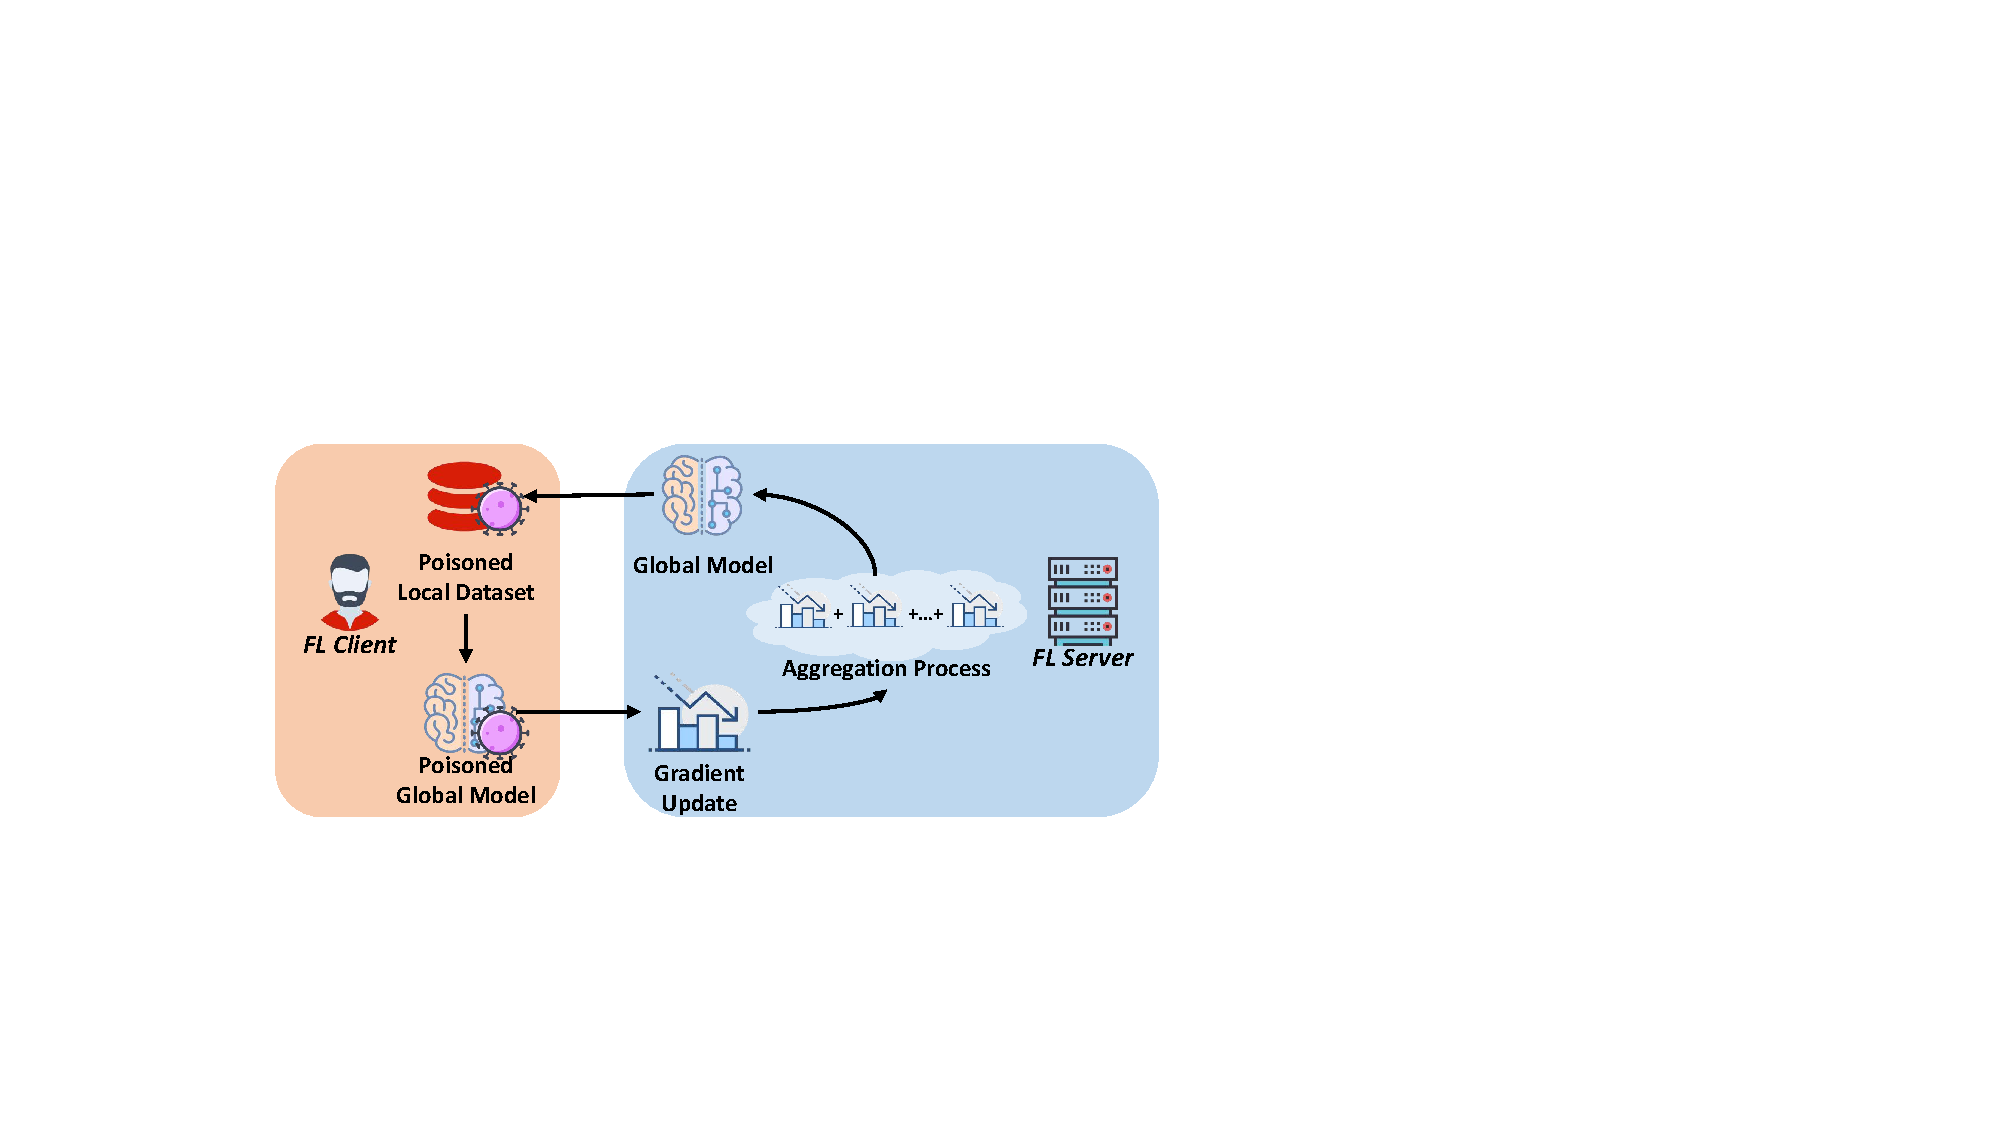
\includegraphics[width=0.5\textwidth]{figures/FLPhish_System.pdf}
  \caption{System Model\&Threat Model.}
  \label{fig_system}
  \end{figure}   
\subsubsection{{FL Server}} FL server $s$ sends a global model to each client at each iteration. After receiving the gradient updates of all the clients, the FL server aggregates the gradient updates for a global update based on FedAvg. After the aggregation process, the FL server updates the global model.

\subsubsection{{FL Client}} Each FL client {$c_{i}$} ($c_{i}$ indicates the $i$th client in FL) keeps the local dataset $d_{i}$ collected by itself. FL client $c_{i}$ uses its local dataset $d_{i}$ to update the model received from the FL server. Then it dispatches the gradient updates of the model back to the FL server. Meanwhile, it repeats the above actions in the whole process of FL until the FL server $s$ stops sending the new model.

\subsection{Threat Model}
The current system still suffers from the Byzantine attacks. Malicious Byzantine client $b$ initiates untargeted Byzantine attacks towards the global model via the label flipping attack in the current system model. Label-flipping requires $b$ to modify the labels of training data and ensure the features of data are unchanging \cite{ref_18_label_flipping}. Byzantine client $b$'s local model is trained with false labels, thus constructing a `poisoned' model with low accuracy. Then Byzantine client $b$ dispatches the false updates of the gradient to the central server. Therefore the false updates of the gradient cause the central server to learn the falsely distilled knowledge from clients. The server $s$'s aggregation process is performed on FedAvg which takes each client $c_{i}$'s dataset $d_{i}$'s size as the aggregation weight for $c_{i}$. This means that a client $c_{i}$ with a larger size of $d_{i}$ gets a larger aggregation weight. Meanwhile FedAvg takes the size of $d_{i}$ declared by $c_{i}$ as $d_{i}$'s real size which means $c_{i}$ can declare a fake size value larger than $d_{i}$'s real size value. If the weight of the malicious clients reaches a threshold, the central server is misguided to produce false predictions.


\subsection{Design Goals}
The key objective of the proposed FLPhish scheme is to provide a robust approach to accurately resist opportunistic untargeted attacks in our Ensemble FL system. Our design goals are given as follows:

\par \textit{1)} Inspired by the idea of ensemble learning, we build a new FL architecture called Ensemble FL. It reduces the network transfer cost and provides more opportunities for us to counter Byzantine attacks in FL.
\par \textit{2)} Our proposed Ensemble FL architecture lacks protection against Byzantine attacks. Since the clients in FL can not be fully trusted, we urgently require an efficient way to tackle malicious Byzantine clients. Thus, we present a phishing-based model to guard against Byzantine attacks in our proposed Ensemble FL system.
\par \textit{3)} To accurately assess clients' behaviors, we further propose an effective Bayesian-based reputation scheme based on our phishing-based model to spot Byzantine attacks compromised by malicious users.
\par \textit{4)} Furthermore, we propose two aggregation algorithms in FLPhish, FLPhish-threshold, and FLPhish-weight to aggregate the predictions of the FL clients, which can further enhance FLPhish's defending ability against Byzantine attacks.


  \begin{figure*}
    \centering
  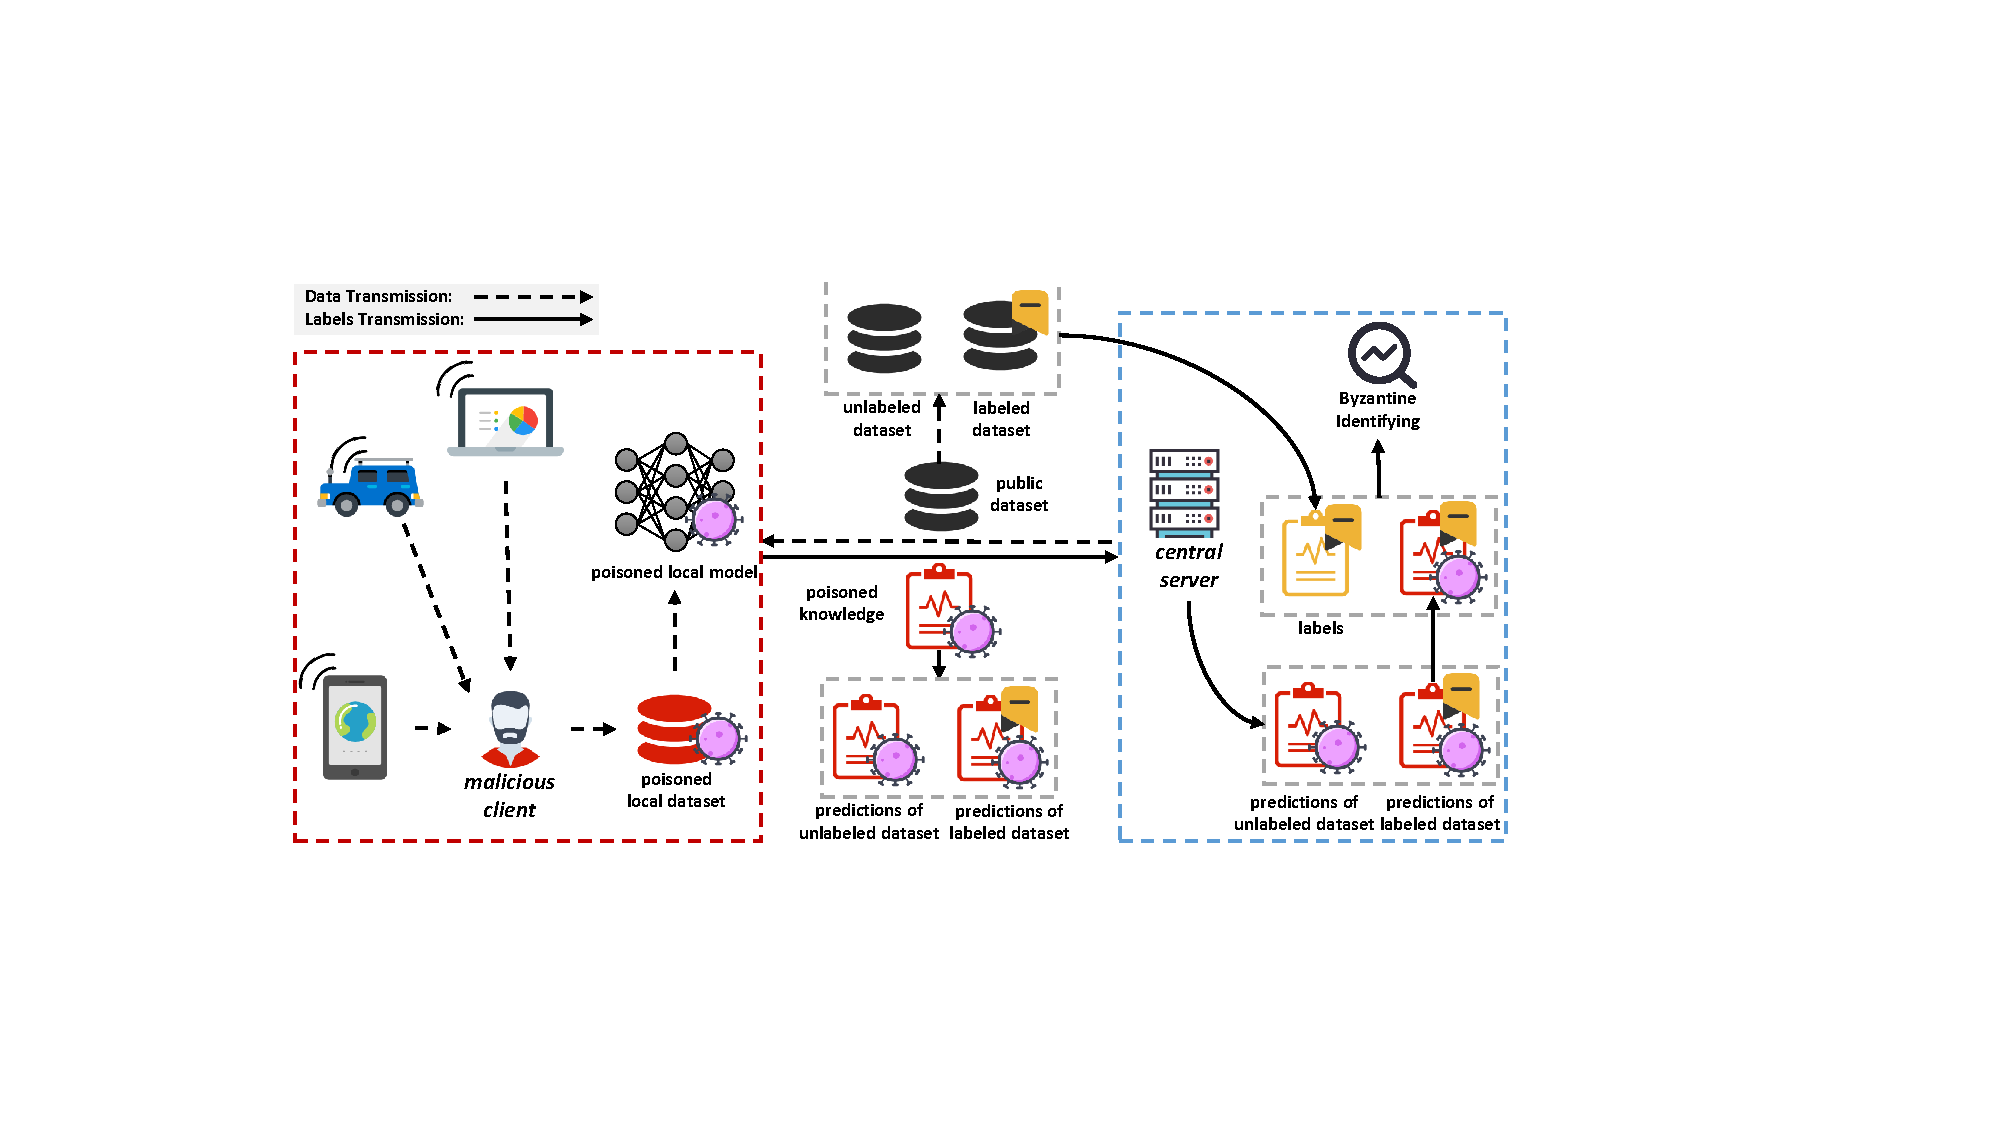
\includegraphics[width=0.95\textwidth]{figures/Figure_FLPhish.pdf}
  \caption{Our Proposed FLPhish Scheme.}
  \label{fig_Phishing}
  \end{figure*}   
  

\section{Proposed FLPhish Scheme}
In this section, we show the proposed FLPhish scheme including the Ensemble Federated Learning, the phishing mechanism, the reputation mechanism, and the aggregation algorithms.

\begin{algorithm}[t]
  \caption{Ensemble FL} %algorithm name
  \label{alg:system}
  \hspace*{0.02in} {\bf Input:} %the input of the algorithm
  the ensemble of clients $C$ with local dataset $d_i$, $i=1,2,3,...,u$; a central server $s$ with unlabeled dataset $D$; number of training iterations $T$; unlabeled batch size $n$;\\
  \hspace*{0.02in} {\bf Output:} %output of the algorithm
  \begin{algorithmic}[1]
    \State $\mathbf{m_i}$ $\gets$ each client $c_i$ train a local model using its own local dataset $d_i$;
    \For{\textit{t=1,2,3,..,,T}}
      \State $s$ selects $D_t$ (containing $n$ samples) from $D$;
      \For{\textit{i=1,2,3,...,u}}
        \State $s \overset{D_{t}}{\rightarrow} c_{i}$;
        \State $c_i$ makes predictions $\mathbf{k_i^t}$ of the $D_t$;
        \State $c_i \overset{\mathbf{k_i^t}}{\rightarrow} s$;
      \EndFor
      \State $Y_t$ = $KnowledgeEnsemble(\mathbf{k_1^t},\mathbf{k_2^t},\mathbf{k_3^t},...,\mathbf{k_u^t})$;
      \State $\mathbf{M}$ = $ModelUpdate(Y_t, D_t, \mathbf{M})$;
    \EndFor \\
    \Return $\mathbf{M}$.
  \end{algorithmic}
\end{algorithm}
\begin{algorithm}[t]
  \caption{KnowledgeEnsemble} %algorithm name
  \label{alg:KnowledgeEnsemble}
  \hspace*{0.02in} {\bf Input:} %input of the algorithm
  the ensemble of ${\mathbf{k_i^t}}_{\left \{ i= 1,2,3,...,u \right \}}$; size of each client's local dataset ${e_i}_{\left \{ i= 1,2,3,...,u \right \}}$; the unlabeled dataset $D_t$ used in $t$th procedure; $\mathbf{\hat{y}^t}$ is the ensembled prediction of dataset $D_t$; $\mathbf{\hat{y}^t_l}$ denotes the prediction of the dataset $D_t$ made by $i$th client;\\
  \hspace*{0.02in} {\bf Output:} %output of the algorithm
  \begin{algorithmic}[1]
    \For{$l=1,2,3,...,n$ ($l=1,2,3,...,n$, denotes the data point in the unlabeled dataset)}
      \State $\mathbf{\hat{k}^t}$ $\gets$ $\sum_{i=1}^{u}\frac{e_i}{\sum_{i=1}^{u}e_i}\mathbf{\hat{k}^t}_i$;
      \State $\mathbf{\hat{y}^t}\gets argmax(\mathbf{\hat{k}^t})$;
    \EndFor \\
    \Return $\mathbf{\hat{y}^t}$.
  \end{algorithmic}

\end{algorithm}

\subsection{Designed Ensemble Federated Learning}
Inspired by ensemble learning, we propose a new FL architecture, called Ensemble FL.
\par Unlike existing FL architecture, which adopts gradient updates for global model updates, we apply an unlabeled dataset preserved by a central server and clients' predictions of it for global aggregation.
\subsubsection{{Client}} Each client {$c_{i}$} ($i$ indicates the number of the client) collects and labels its local data, which is from the personal computer, smartphone, smart cars and etc. The collected data is labeled and preprocessed by {$c_{i}$}, and {$c_{i}$} adopts the preprocessed local dataset to train its local model. When receiving a public dataset, {$c_{i}$} utilizes its local model to make predictions for the public dataset and return the predictions to the central server {$s$}.
\subsubsection{{Central server}} Central server {$s$} is responsible for making a public dataset and building a global model. The public dataset consists of a variety of unlabeled data. The dataset is collected by {$s$} or produced by it (such as using GAN to generate data). After the construction of the public dataset, {$s$} sends the public dataset to the clients. Each client {$c_{i}$} sends its predictions about the public dataset back to {$s$}. After receiving all the predictions, {$s$} aggregates the predictions. Then {$s$} employs the aggregated results and the public dataset to train the global model.

\par This system model demonstrates a variety of advantages over traditional FL architectures:
\begin{itemize}

  \item The selection of the global model and each client's local model is restricted to the same type of neural architecture in traditional FL. Nevertheless, in our system, deploying different types of neural architectures is allowed by applying the distilled knowledge (the predictions of the unlabeled data produced by the clients). Different selected features in different clients are permitted as well.
  \item The overhead and latency of the communication process are significantly reduced compared to the traditional FL architecture. Transferring data is much faster than transferring gradient updates. 
  \item The design of Ensemble FL can prevent the backdoor attack in FL. The detail of theoretical proof will be in the next section.
\end{itemize}
      
\subsection{Theoretical Proof about Defending Backdoor Attack}
Backdoor attackers in FL need to hide some triggers in their local dataset. Each backdoor attacker adopts the preprocessed local dataset to update the global model it received from the FL server. Then it transfers the poisoned model updates which contain the information of the triggers to the FL server. After receiving the poisoned model updates, the FL server will update the global model using the poisoned model updates of the backdoor attackers. After the updating, the FL server's model will misclassify the data with the triggers to the chosen label of backdoor attackers.
\par While in Ensemble FL, the model update is replaced from gradient update to the predicted labels of the public dataset. First, the dimension of the model update is reduced so that the information of triggers in backdoor attackers' local dataset can not be transferred. Second, the public dataset is produced by the central server, therefore making backdoor attackers impossible to hide the triggers in the public dataset. As a consequence, the backdoor attack is unable to achieve in the setting of Ensemble FL.








\subsection{Phishing Mechanism-based Detection}
The proposed Ensemble FL still confronts the threat of Byzantine attacks. Malicious clients can manipulate their local model via label flipping. They mislabel the local dataset to build a `poisoned' local model. When malicious clients receive unlabeled data from the central server, they manufacture false predictions (called poisoned knowledge) and send these false predictions to the central server. Subsequently, the central server aggregates the false predictions as the labels of the unlabeled dataset. Then central server trains the global model using these unlabeled datasets with the false aggregation predictions. Therefore, a flawed global model is manufactured. Inspired by the idea of ensemble learning, we consider utilizing the labeled data in the architecture of Ensemble FL to cope with Byzantine attacks. We called labeled data `bait'.
  \subsubsection{\ul{Local Model Training}} The ensemble of clients $C=\left \{ c_{1},c_{2},...,c_{n-1},c_{n} \right \}$. Each client $c_i$ possesses a local dataset $d_i$. At the beginning of the Ensemble FL, $c_{i}$ utilizes its local dataset $d_i$ to train a local model $\mathbf{m_i}$ as
  \begin{equation}
    \mathbf{m_i}=Train(d_i).
  \end{equation}
  \subsubsection{\ul{Dataset Transferring}} Central server $s$ selects $n$ samples of data $D_t$ from unlabeled dataset $D$ and $m$ samples of data $B_t$ from labeled dataset $B$ randomly. Then $s$ sends $D_t$ and $B_t$ to each client $c_i$ as
  \begin{equation}
    s \overset{{D_{t},B_{t}}}{\rightarrow} c_{i}.
  \end{equation}
  \subsubsection{\ul{Label Predicting}} Each client $c_i$ predicts the labels of the unlabeled data $D_t$ and the labeled data $B_t$:
  \begin{equation}
    \mathbf{k_i^t}=Predict(D_t, B_t, \mathbf{m_i})
  \end{equation}
  ($c_i$ can not distinguish between $D_t$ and $B_t$) via the local model trained by itself in Step 1  and sends its prediction back to the central server as the distilled knowledge $\mathbf{k_i^t}$:
  \begin{equation}
    \mathbf{k_i^t}=\begin{vmatrix}
      p_{1,1} & p_{1,2} & \cdots  & p_{1,g-1} & p_{1,g}\\ 
      \vdots  & \vdots & \ddots  & \vdots & \vdots\\ 
      p_{n,1} & p_{n,2} & \cdots  & p_{n,g-1} & p_{n,g}
      \end{vmatrix}.
  \end{equation}

  \begin{algorithm}[t]
    \caption{Phishing Mechanism} 
    \hspace*{0.02in} {\bf Input:} 
    the ensemble of clients $C$ with local dataset $d_i$, $i=1,2,3,...,u$; a central server $s$ with unlabeled dataset $D$ and labeled dataset $B$; number of training iterations $T$; unlabeled batch size $n$;labeled batch size $m$.\\
    \hspace*{0.02in} {\bf Output:} 
    output result
    \begin{algorithmic}[1]
      \State $\mathbf{m_i}$ $\gets$ each client $c_i$ train a local model using its own local dataset $d_i$.
      \For{\textit{t=1,2,3,..,,T}}
        \State $s$ selects $D_t$ (containing $n$ samples) from $D$ and $B_t$ (containing $m$ samples) from $B$.
        \For{\textit{i=1,2,3,...,u}}
          \State $s$ sends $D_t$ and $B_t$ to $c_i$.
          \State $c_i$ makes predictions $\mathbf{k_i^t}$ of the $D_t$ and $B_t$.
          \State $c_i$ sends $\mathbf{k_i^t}$ to $s$.
          \State $s$ calculates the accuracy $a_i^t$ of the predictions of $B_t$ made by $c_i$ in $t$th procedure.
          \If{$a_i^t > r_q$}
            \State $q_i = 1$.
            \For{\textit{j=i,i+1,i+2,...,u-1}}
              \State $(d,c,\mathbf{k^t},q,a^t)_j \gets (d,c,\mathbf{k^t},q,a^t)_{j-1}$.
            \EndFor
          \EndIf
        \EndFor
        \State $\mathbf{K_t}$ = $KnowledgeEnsemble(\mathbf{k_1^t},\mathbf{k_2^t},\mathbf{k_3^t},...,\mathbf{k_u^t})$.
        \State $\mathbf{M}$ = $ModelUpdate(\mathbf{K_t}, D_t, \mathbf{M})$.
      \EndFor
      \State\Return $\mathbf{M}$
    \end{algorithmic}
    \end{algorithm}


  Unlike benign clients, malicious clients return the false prediction as the distilled knowledge to central server $s$.
  \subsubsection{\ul{Byzantine Identifying}} Accepting the distilled knowledge from each client $c_i$, $s$ extracts the predictions of the \textit{`bait'} from $\mathbf{k_i^t}$, and calculates the accuracy of the predictions via the true label of the \textit{`bait'}:
  \begin{equation}
    a_i^t=AccuracyCal(\mathbf{k_i^t}, B_t).
  \end{equation}
  Then $s$ identifies those clients who hold a low value of accuracy and distinguishes as malicious clients.
  \subsubsection{\ul{Global Model Updating}} After identifying the malicious clients within all clients, $s$ aggregate the knowledge $\mathbf{\hat{k}^t}$ from all clients as
  \begin{equation}
    \mathbf{\hat{k}^t}=\sum_{i=1}^{u}\frac{e_i}{\sum_{i=1}^{u}e_i}\mathbf{\hat{k}^t}_i.
  \end{equation}
  Then the server $s$ uses the aggregated knowledge $\mathbf{\hat{k}^t}$ to get the labels
  \begin{equation}
    \mathbf{\hat{y}^t}\gets argmax(\mathbf{\hat{k}^t}).
  \end{equation} 


  



\subsection{Bayesian Inference-based Reputation Mechanism}
Server $s$ maintains a reputation list which records the reputation of all the clients $C$ in the model. Let $X_i$ be the reputation of the $c_i$ client which represents $s$'s belief that how likely client $c_i$ is a Byzantine client. The computation of $X_i$ is based on the accuracy $a_i^t$ of client $c_i$ from the 1st iteration to the $t$th iteration. Every time a new update of client $c_i$ comes to server $s$, $s$ uses the accuracy $a_i^t$ to update the $X_i$.
\par Initially, the reputation is neutral. Each client $c_i$ is considered a benign client by server $s$ with a probability of 50\%. When a new update $\mathbf{k_i^t}$ comes to the server $s$, the reputation is updated by the $s$. When the reputation is lower than the threshold $r$, $s$ considers the client $c_i$ as a Byzantine client officially and discards the update coming from the client $c_i$. The updates of the client $c_i$ are reconsidered in the aggregation when the $X_i$ exceeds the threshold $r$.
\par We employ Bayesian inference to construct our reputation mechanism. Each data prediction made by client $c_i$ faces two situations: wrong predictions or correct predictions. Thus, the use of binomial parameter distributions becomes a natural choice for our reputation mechanism. Let $Y_i$ be the event that the number of wrong predictions and correct predictions made by client $c_i$ is $\alpha_i$ and $\beta_i$. Given $X_i=\gamma_i$, then the conditional probability is 
\begin{equation}
    Pr(Y_i|X_i=\gamma _i)=\left ( \frac{\alpha _i+\beta _i}{\alpha _i} \right )\gamma {_{i}}^{\alpha_i}\left ( 1-\gamma_{i} \right )^{\beta_{i}}\label{equation_1}.
\end{equation}
$\alpha_i$ and $\beta_i$ is the available evidence for the estimation of the $X$. $\gamma_i$ is unknown. Eq. \ref{equation_1} indicates the likelihood function for $X$. According to Bayesian inference we compute the posterior probability as
\begin{equation}
    Pr(X_i=\gamma _i|Y_i)=\frac{Pr\left ( Y_{i}|X_{i}=\gamma_{i} \right )Pr(X_{i}=\gamma_{i})}{\int_{0}^{1}Pr\left ( Y_{i}|X_{i}=x \right )Pr(X_{i}=x)dx}\label{equation_2}.
\end{equation}
As the posterior probability function is given by our analysis, the final value for the expectation value of reputation $X$ is computed as
\begin{equation}
    E(X)=\int_{0}^{1}\frac{Pr\left ( Y_{i}|X_{i}=\gamma_{i} \right )Pr(X_{i}=\gamma_{i})}{\int_{0}^{1}Pr\left ( Y_{i}|X_{i}=x \right )Pr(X_{i}=x)dx}\gamma_{i}d\gamma_{i}\label{equation_3}.
\end{equation}
Furthermore, we decide to use the binomial parameter beta distribution to describe the distribution of X. Assume X is a random variable of the beta distribution with the parameters $(\alpha, \beta)$. Therefore the density function is
\begin{equation}
    f(x,\alpha,\beta)=\frac{1}{B(\alpha,\beta)}x^{\alpha-1}(1-x)^{\beta-1}\label{equation-4}.
\end{equation}
$B$ function is the beta function. Therefore we compute the expectation of $X$ as
\begin{equation}
    E(x)=\frac{\alpha}{\alpha+\beta}.
\end{equation}

Therefore server ${s}$ can easily compute the reputation of the client ${c_{i}}$ as ${E(x_{i})=\frac{\alpha_{i}}{\alpha_{i}+\beta_{i}}}$. We set the initial value of the reputation to 50\% by set the value of ${\alpha}$ and ${\beta}$ to 1. This indicates that the probability of being benign client and malicious client are equal for client ${c_{i}}$. When a new iteration of FL is accomplished, ${\alpha_{i}}'$ and ${\beta_{i}}'$ are provided as the new evidence for the computation of the reputation. The parameters are updated as ${(\alpha_{i}+{\alpha_{i}}',\beta_{i}+{\beta_{i}}')}$. Then the reputation is given by
\begin{equation}
    {E(x_{i})}'=\frac{\alpha_{i}+{\alpha_{i}}'}{\alpha_{i}+{\alpha_{i}}'+\beta_{i}+{\beta_{i}}'}.
\end{equation}



\subsection{Aggregation Algorithms}
Based on our reputation mechanism, we propose our Byzantine-tolerant aggregation algorithms: FLPhish-threshold and FLPhish-weight.
\subsubsection{{FLPhish-threshold}}
FLPhish-threshold functions as the aggregation rules identify the clients whose reputation is lower than the reputation threshold. Then the server discards the Byzantine clients and aggregates the global model using the survived clients' updates. Server identifies the client ${c_{i}}$ whose reputation is lower than the threshold $\tau$ as Byzantine clients, and given them a aggregation weight as
\begin{equation}
  \omega_{i}=\begin{cases}
    1 & \text{ if } x\geq \tau \\ 
    0 & \text{ if } x< \tau 
    \end{cases}.
\end{equation} 
The aggregated knowledge is given by
\begin{equation}
  \mathbf{\hat{k}^t}=\sum_{i=1}^{u}\frac{e_i}{\sum_{i=1}^{u}e_i}\mathbf{\hat{k}^t}_i\times \omega_{i},
\end{equation}
\begin{equation}
  \mathbf{\hat{y}^t}\gets argmax(\mathbf{\hat{k}^t}).
\end{equation} 
\subsubsection{{FLPhish-weight}}
Unlike FLPhish-threshold, FLPhish-weight does not discard the potential Byzantine clients' updates. On the contrary, it enables the Byzantine clients to participate the aggregation using its reputation value as the aggregation weight. Due to our reputation mechanism, the Byzantine clients are offered a low value of reputation, so it has a lower influence on aggregation.
Give a reputation list $R=\left | x_{1},x_{1},x_{1},\cdots ,x_{n-1},x_{n} \right |$, the prediction results is 
  \begin{equation}
    \mathbf{k_i^t}=\begin{vmatrix}
      p_{1,1} & p_{1,2} & \cdots  & p_{1,g-1} & p_{1,g}\\ 
      \vdots  & \vdots & \ddots  & \vdots & \vdots\\ 
      p_{n,1} & p_{n,2} & \cdots  & p_{n,g-1} & p_{n,g}
      \end{vmatrix},
  \end{equation}
  FLPhish-weight computes the aggregated knowledge, which is
    \begin{equation}
    \mathbf{\hat{k}^t}=\sum_{i=1}^{u}\frac{e_i}{\sum_{i=1}^{u}e_i}\mathbf{\hat{k}^t}_i\times x_{i}.
  \end{equation}
  Then the server $s$ uses the aggregated knowledge $\mathbf{\hat{k}^t}$ to get the labels
  \begin{equation}
    \mathbf{\hat{y}^t}\gets argmax(\mathbf{\hat{k}^t}).
  \end{equation} 
In a word, FLPhish-weight does not identify the Byzantine clients but treats the clients with a low reputation as `bad' clients and give them lower weight.

% Please add the following required packages to your document preamble:
% \usepackage{booktabs}
\begin{table}[t]

  \renewcommand\arraystretch{1.5}
  \centering
  \caption{Parameter Settings}
  \resizebox{0.5\textwidth}{!}{
  \label{tab:my-table}
  \begin{tabular}{ll}
    \bottomrule
    \textbf{Parameter}                    & \textbf{Parameter Value}              \\ \hline
    Client Number                         & 50 clients                                \\ \hline
    Sample Total Number                   & 60000 samples                             \\ \hline
    \multirow{2}{*}{Client Sample Number} & 800 training samples                      \\
                                          & 200 test samples                          \\ \hline
    \multirow{2}{*}{Server Sample Number} & 8000 unlabeled samples                    \\
                                          & 2000 labeled samples                      \\ \hline
    Round Number                          & 10 iterations                                 \\ \hline
    \multirow{2}{*}{Round Sample Number}  & 800 unlabeled samples                     \\
                                          & 200 labeled samples                       \\ \hline
    Deep Learning Model                   & Residual Networks                         \\ \hline
    Byzantine Fractions $p$               & 0,0.1,0.2,0.3,0.4,0.5,0.6,0.7,0.8,0.9     \\ \hline
    Imbalance Degree $q$                  & 0.1,0.2,0.5,0.6,0.7,0.8               \\ \hline
    Dataset $d$                         & MNIST,Fashion-MNIST,CIFAR-10              \\ \hline
    \end{tabular}
}
\end{table}



\section{Performance Evaluation}
In this section, we experimentally evaluate our FLPhish against untargeted attacks under different conditions. Furthermore, we compare FLPhish's performance with FedAvg, Median \cite{ref_13_defense}, and Trimmed Mean \cite{ref_13_defense}'s performance, and the evaluation results show that FLPhish outperforms FedAvg in defending against Byzantine attacks.

\begin{figure*}[!htp]
  \centering
    \subfigure[$q=0.1$]{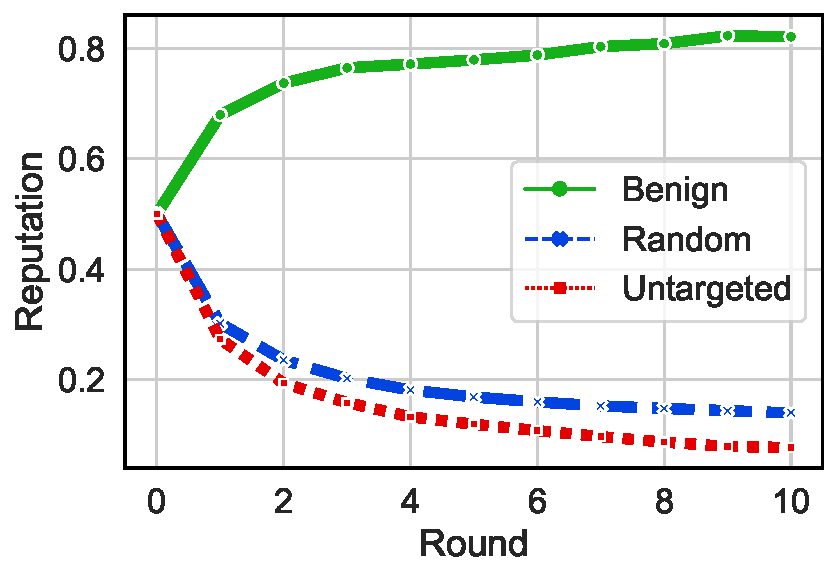
\includegraphics[width=0.245\textwidth]{figures/rep_mnist_imbalance_1.pdf}}
    \subfigure[$q=0.2$]{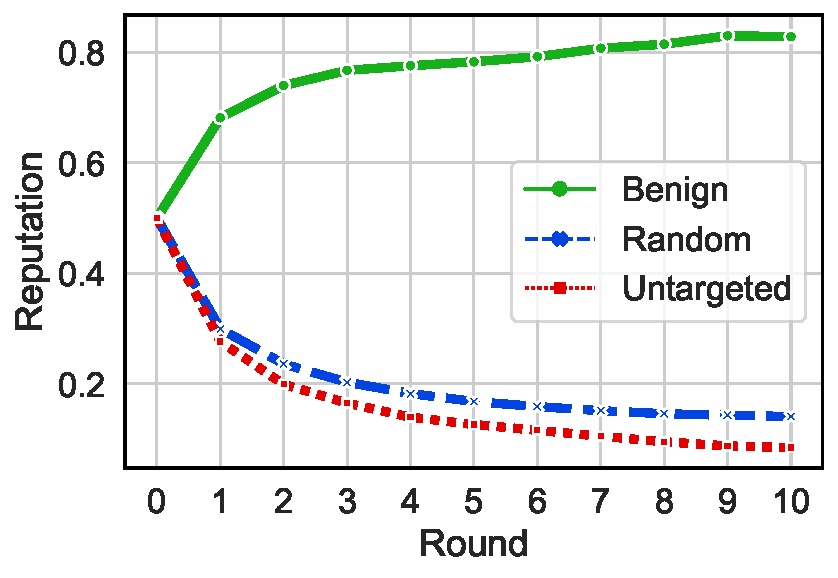
\includegraphics[width=0.245\textwidth]{figures/rep_mnist_imbalance_2.pdf}}
    \subfigure[$q=0.5$]{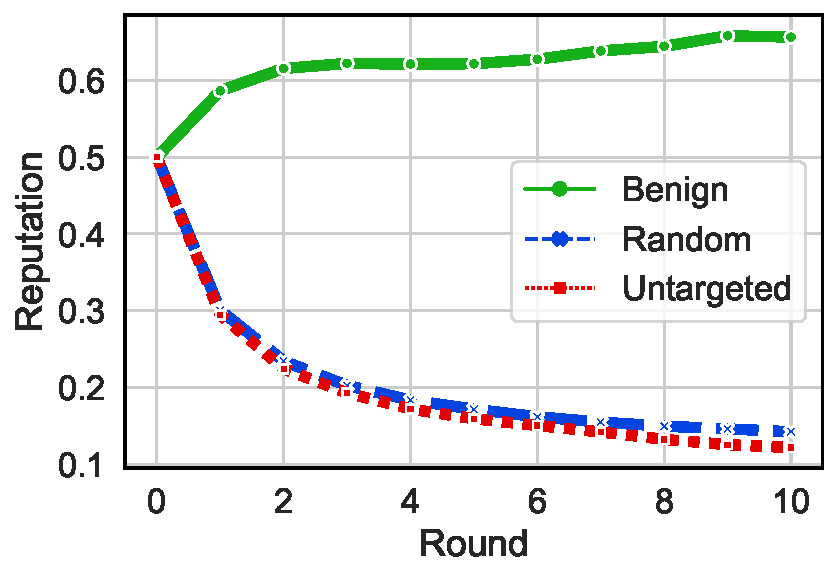
\includegraphics[width=0.245\textwidth]{figures/rep_mnist_imbalance_5.pdf}}
    \subfigure[$q=0.8$]{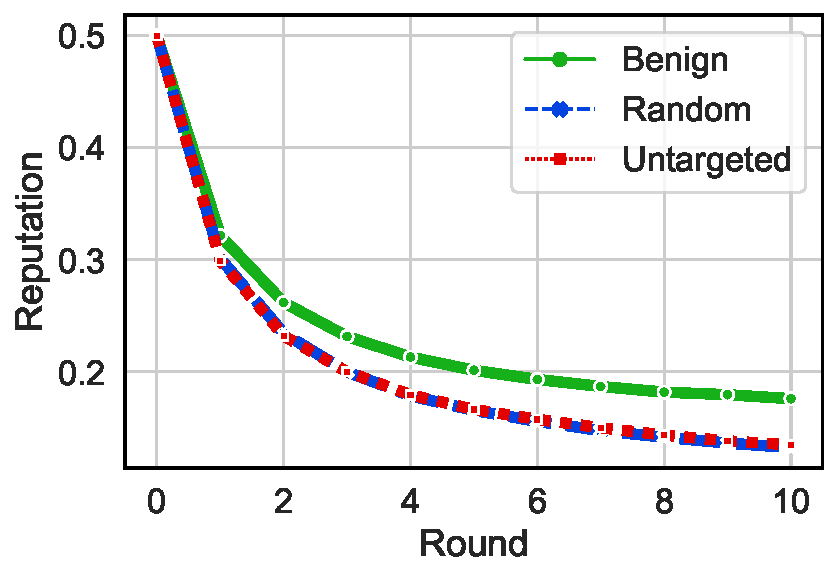
\includegraphics[width=0.245\textwidth]{figures/rep_mnist_imbalance_9.pdf}}
  \\
  \caption{Reputation values of experiments on MNIST on different imbalance degrees.}
  \label{fig_exp_mnist-reputation}
  \vspace{0.2in}
\end{figure*}

\begin{figure*}[!htp]
  \centering
    \subfigure[$q=0.1$]{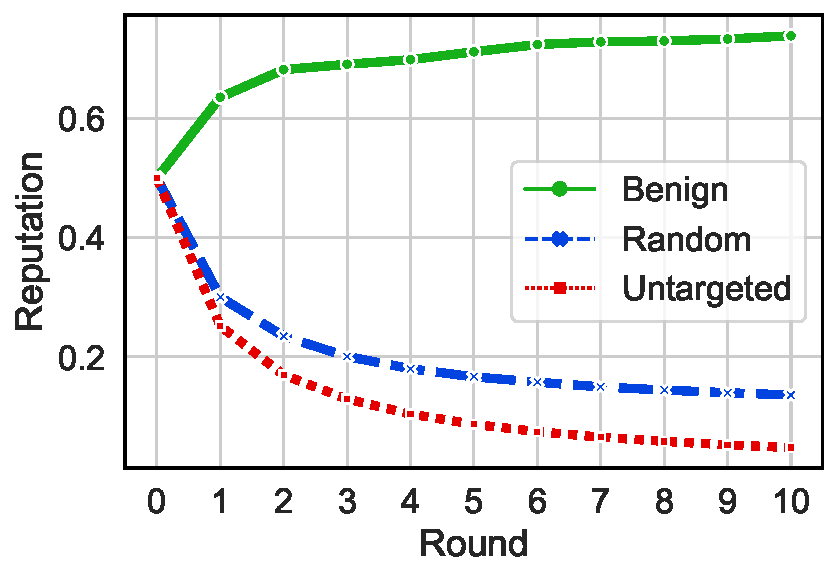
\includegraphics[width=0.245\textwidth]{figures/rep_fashion_imbalance_1.pdf}}
    \subfigure[$q=0.2$]{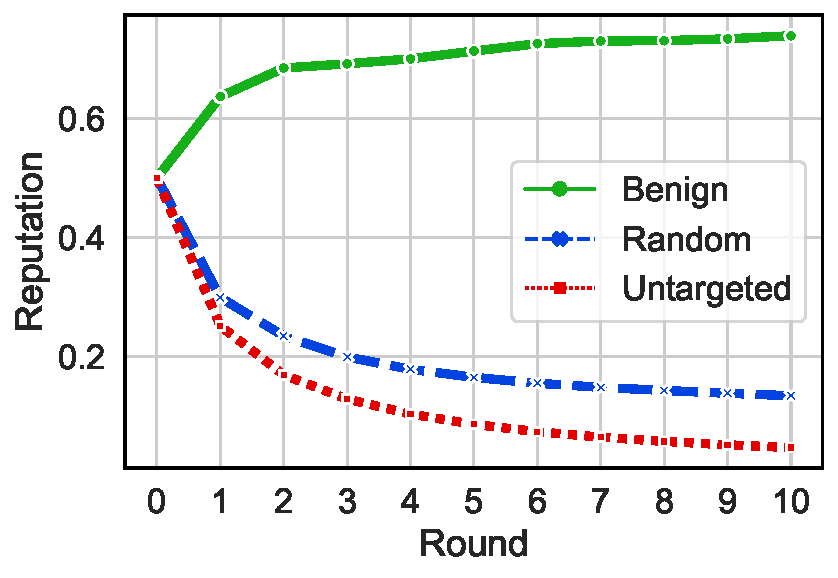
\includegraphics[width=0.245\textwidth]{figures/rep_fashion_imbalance_2.pdf}}
    \subfigure[$q=0.5$]{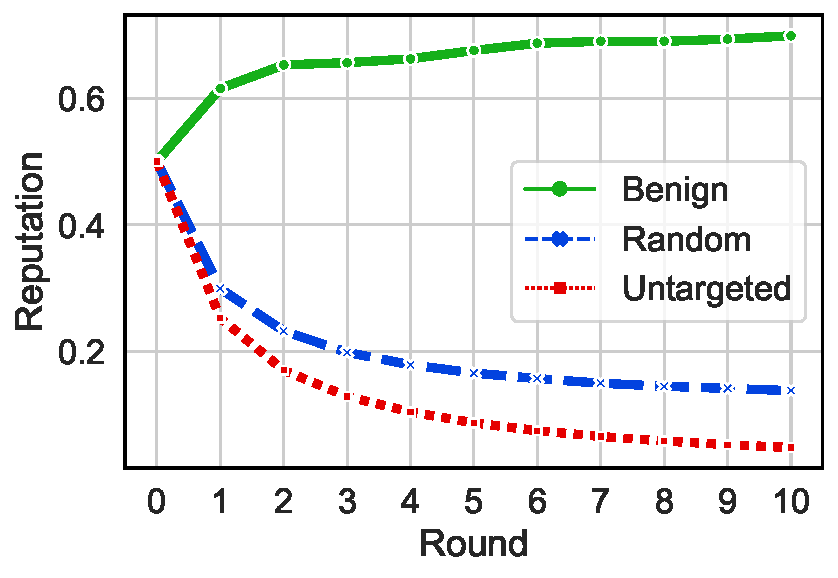
\includegraphics[width=0.245\textwidth]{figures/rep_fashion_imbalance_5.pdf}}
    \subfigure[$q=0.8$]{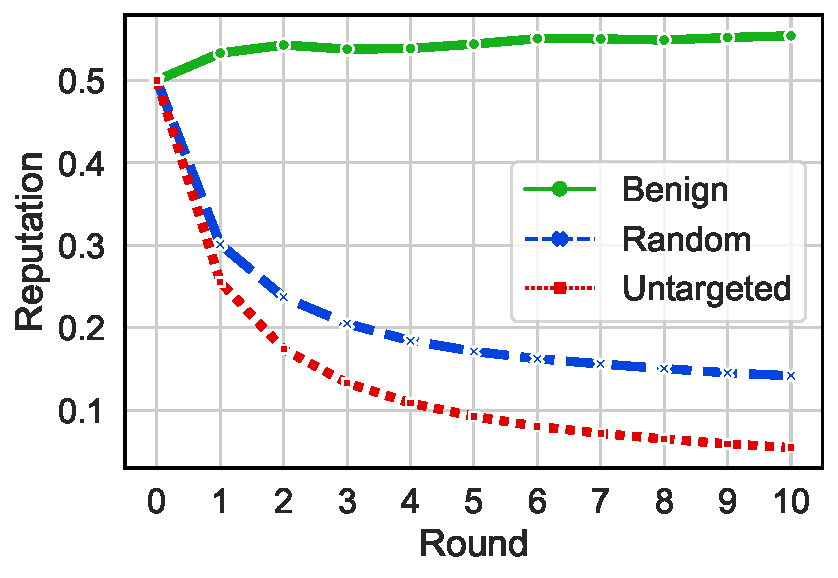
\includegraphics[width=0.245\textwidth]{figures/rep_fashion_imbalance_9.pdf}}
  \\
  \caption{Reputation values of experiments on Fashion-MNIST on different imbalance degrees.}
  \label{fig_exp_fashion_reputation}
  \vspace{0.2in}
\end{figure*}

\begin{figure*}[!htp]
  \centering
    \subfigure[{$q=$}0.1]{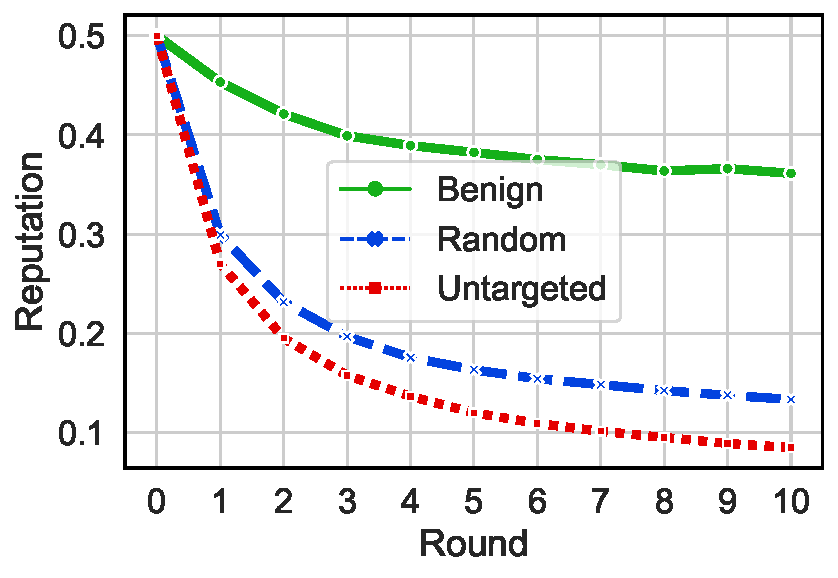
\includegraphics[width=0.245\textwidth]{figures/rep_cifar_imbalance_1.pdf}}
    \subfigure[{$q=$}0.2]{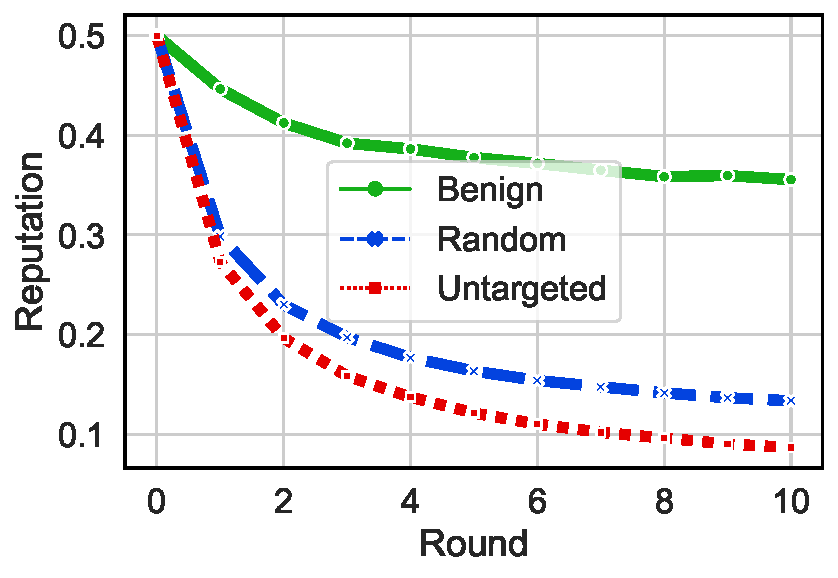
\includegraphics[width=0.245\textwidth]{figures/rep_cifar_imbalance_2.pdf}}
    \subfigure[{$q=$}0.5]{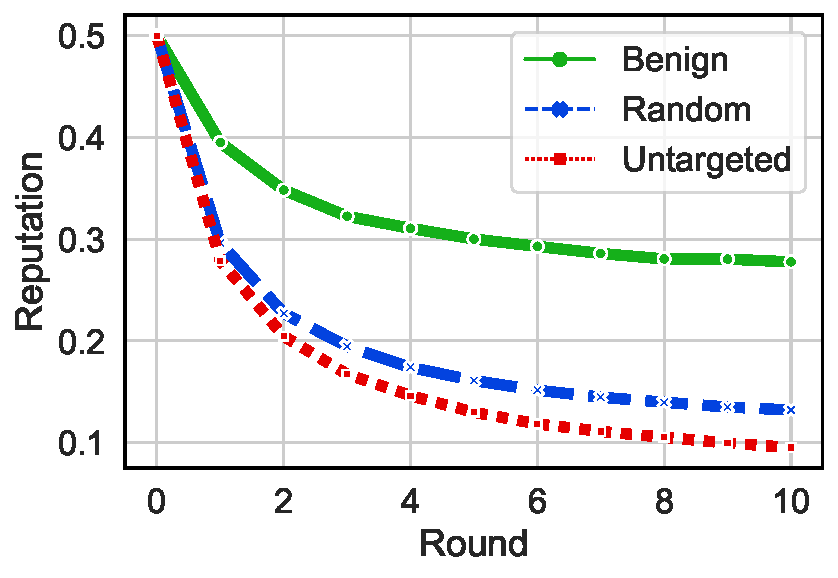
\includegraphics[width=0.245\textwidth]{figures/rep_cifar_imbalance_5.pdf}}
    \subfigure[{$q=$}0.8]{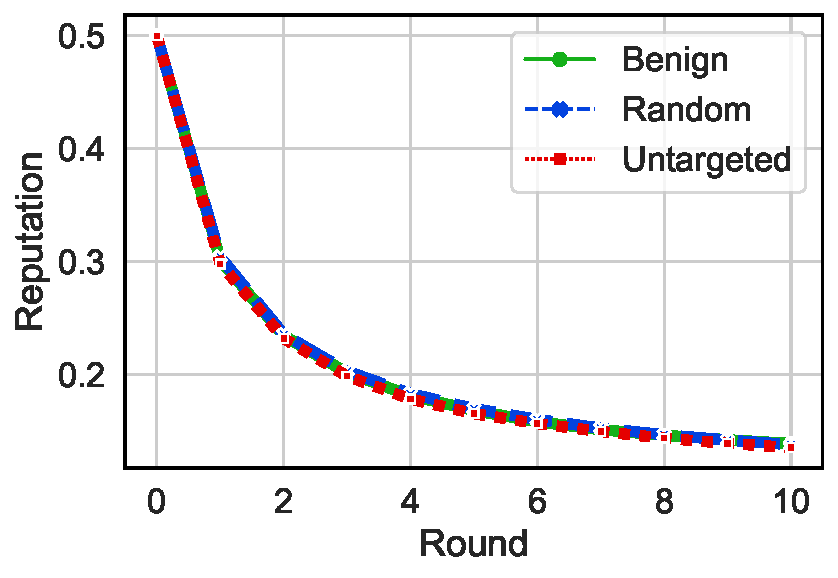
\includegraphics[width=0.245\textwidth]{figures/rep_cifar_imbalance_9.pdf}}
  \\
  \caption{Reputation values of experiments on CIFAR-10 on different imbalance degrees.}
  \label{fig_exp_cifar_reputation}
  \vspace{0.2in}
\end{figure*}

\subsection{Experiment Setup}


  \subsubsection{{\textit{The fraction {$p$} of Byzantine clients}}} We evaluate our FLPhish under the circumstances of different fractions $p$ of Byzantine clients: 0 (no Byzantine clients), 0.1, 0.2, 0.3, 0.4, 0.5, 0.6, 0.7, 0.8, 0.9.
  \subsubsection{{\textit{The imbalance degree {$q$} of the data}}} According to the previous research \cite{ref_06_model}, we distribute the data in a dataset among all the clients. Giving $M$ classes of data in a dataset, we split the clients into $M$ groups. A client $c$ in group $m$ is provided with data where data $m$ accounts for over $q$ percent. Within the same group, data are uniformly distributed among all the clients. The parameter $q$ controls the distribution inference of clients' local training data. If $q=\frac{1}{M}$, the clients' local training data are independent and identically distributed. We evaluate our FLPhish on three different $q$: 0.1 (IID), 0.2, 0.5, 0.6, 0.7, and 0.8.
  \subsubsection{{\textit{The number of clients}}} The number of clients is set to be 50 in our experiment.
  \subsubsection{{\textit{The local CNN model used by clients}}} ResNet is employed to perform deep learning tasks in our local client.
  \subsubsection{{\textit{The datasets {$d$}}}} We take three different datasets as our experiment datasets: \begin{itemize}
      \item MNIST: MNIST is a 10-class digit image classification dataset consisting of 60,000 training examples and 10,000 testing examples.
      \item Fashion-MNIST: Fashion-MNIST is a 10-class fashion image classification dataset. It has a predefined training set of 60,000 fashion images and a testing set of 10,000 fashion images.
      \item CIFAR-10: CIFAR-10 is a color image classification dataset. It consists of predefined 50,000 training examples and 10,000 testing examples. Each example belongs to one of the 10 classes.
  \end{itemize} 





  \begin{figure*}[!htp]
    \centering
    \subfigure[Byzantine Fraction 0.9 \& Imbalance Degree 0.2 \& Random Attack]{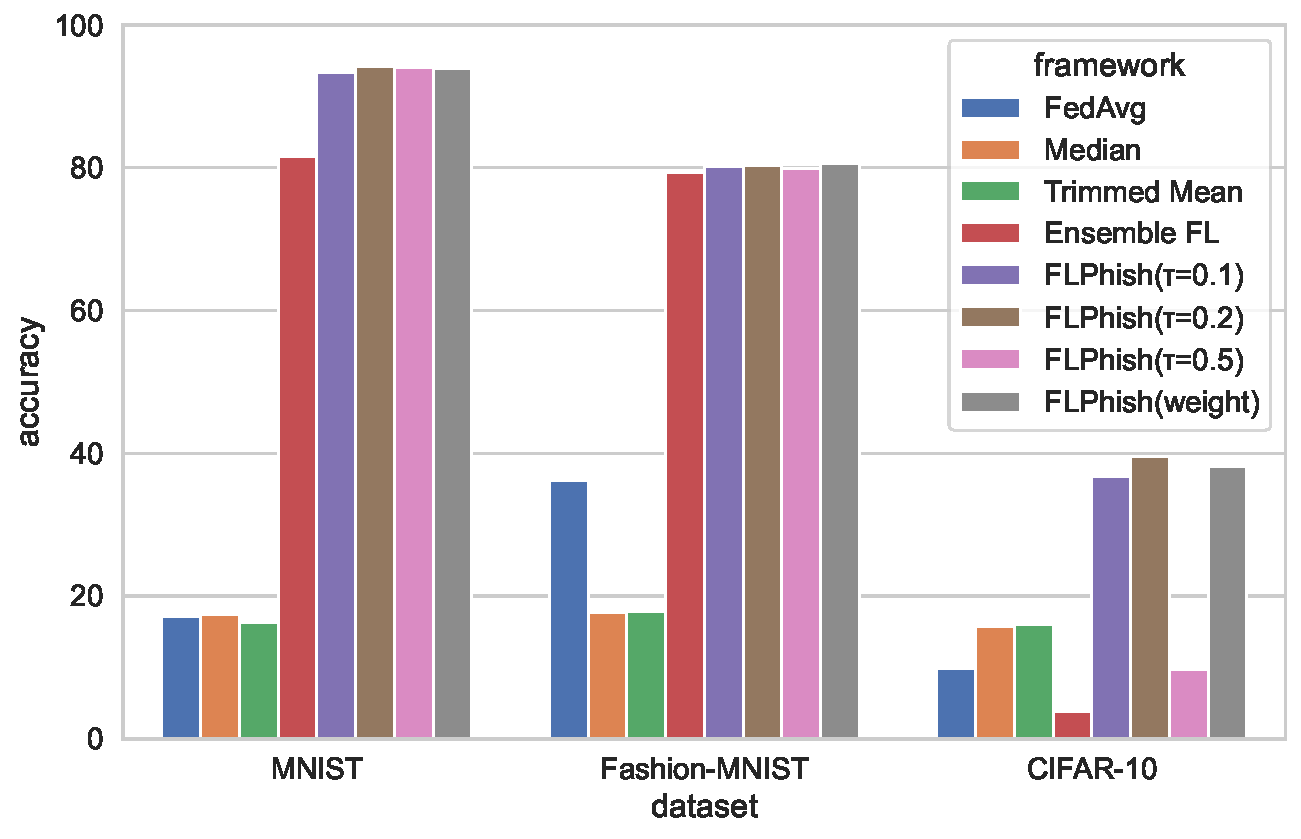
\includegraphics[width=0.48\textwidth]{figures/bar_byzantines_random_bar.pdf}}
    \subfigure[Byzantine Fraction 0.9 \& Imbalance Degree 0.2 \& Untargeted Attack]{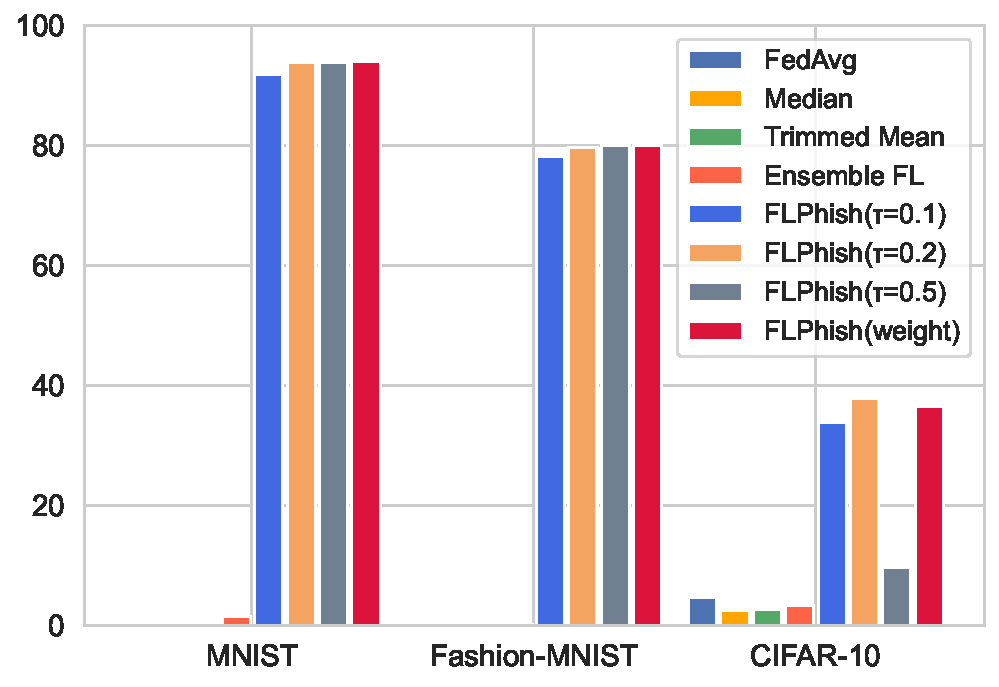
\includegraphics[width=0.48\textwidth]{figures/bar_byzantines_untargeted_bar.pdf}}
    \subfigure[Byzantine Fraction 0.5 \& Imbalance Degree 0.8 \& Random Attack]{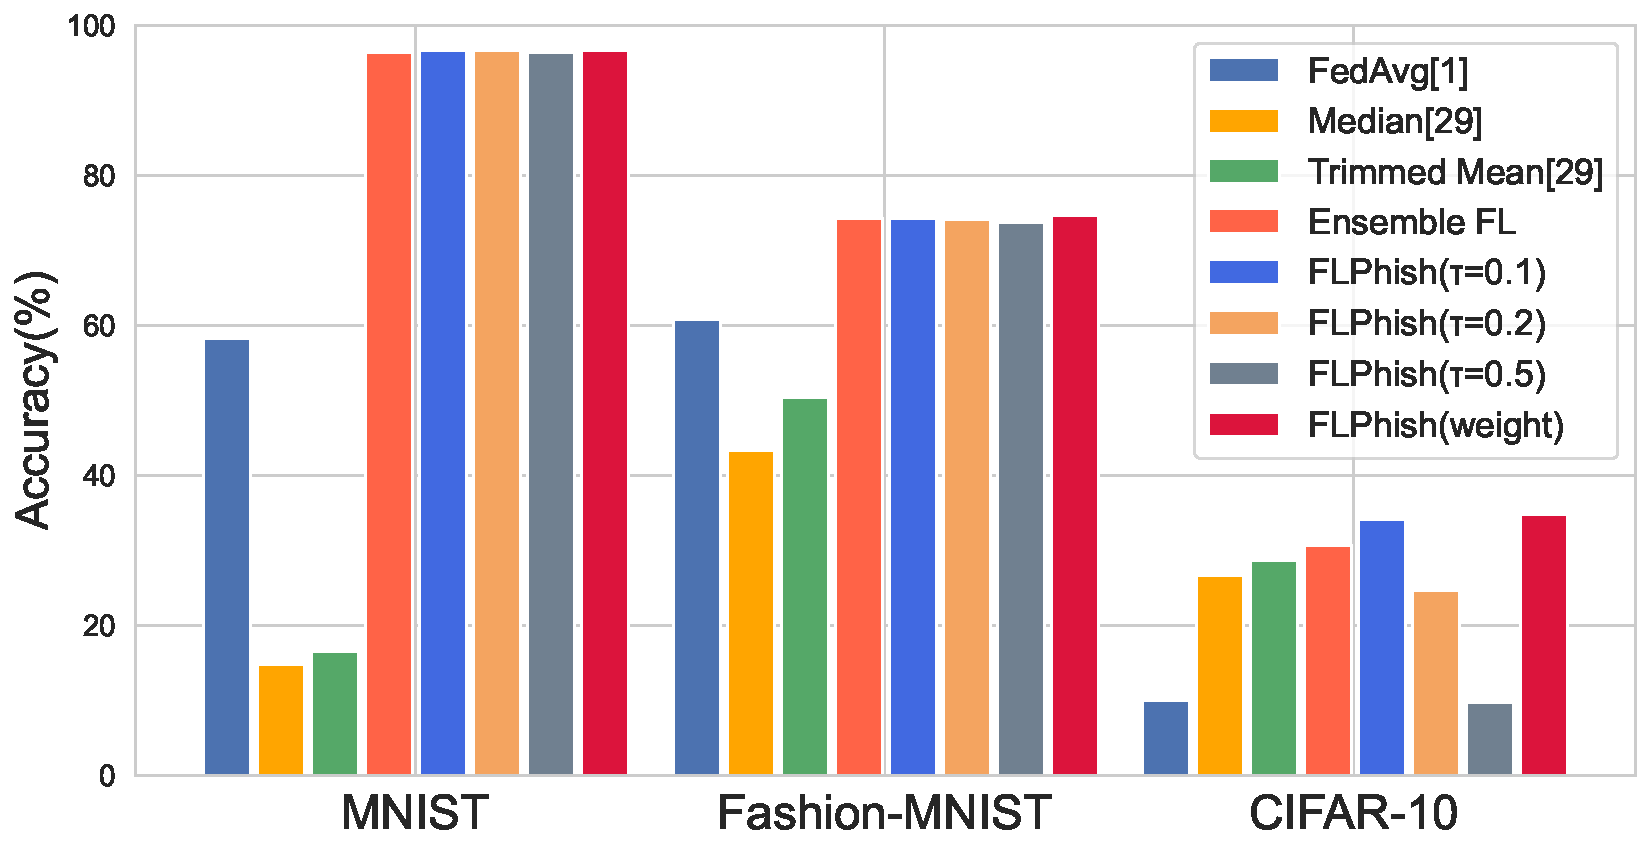
\includegraphics[width=0.48\textwidth]{figures/bar_imbalances_random_bar.pdf}}
    \subfigure[Byzantine Fraction 0.5 \& Imbalance Degree 0.8 \& Untargeted Attack]{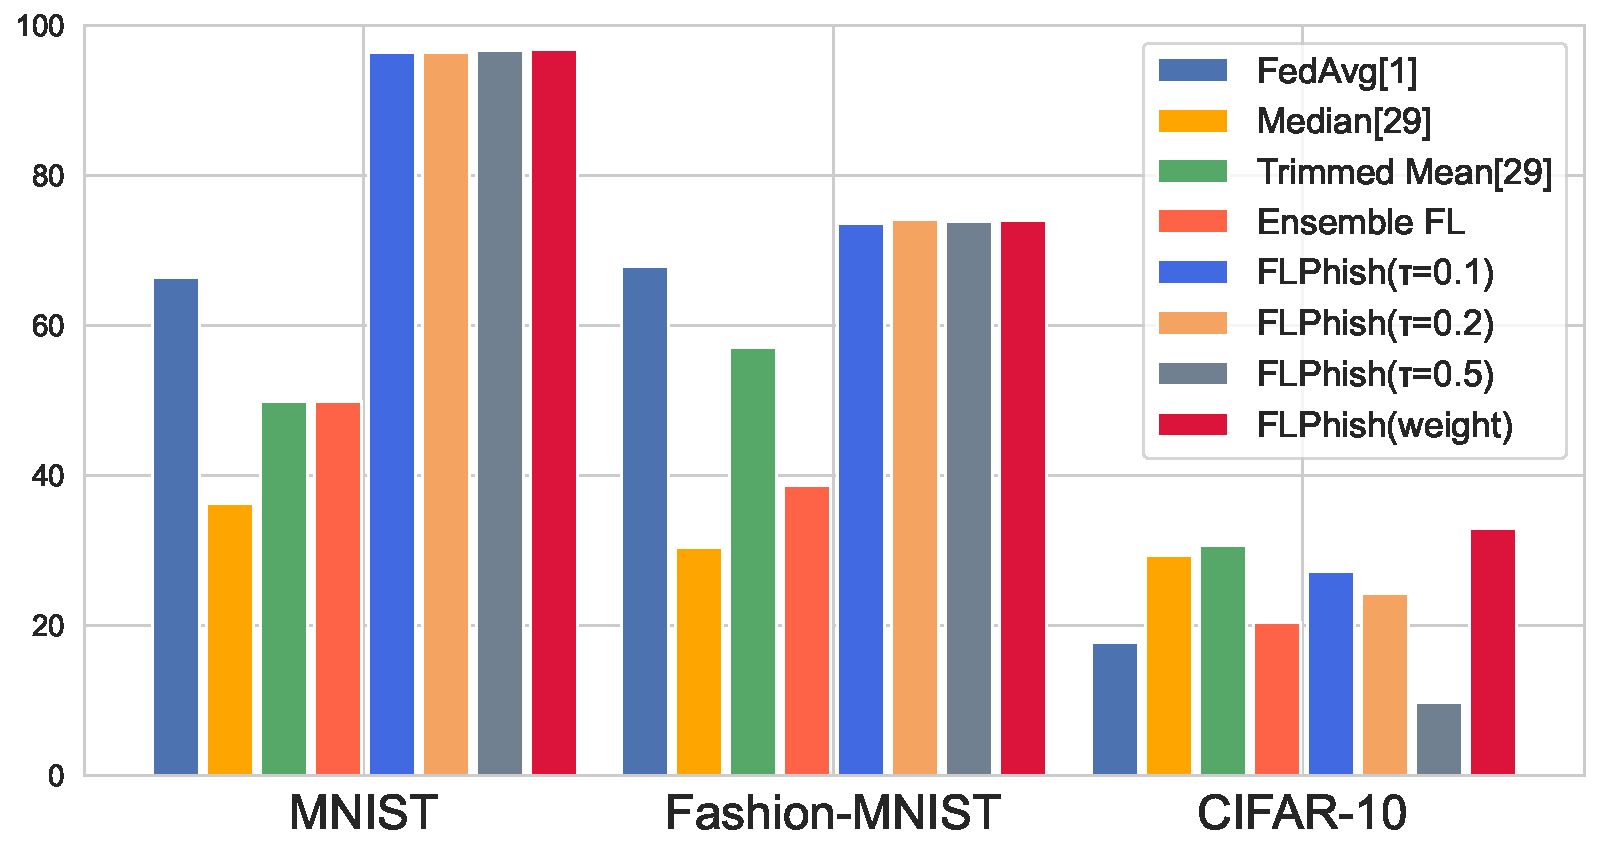
\includegraphics[width=0.48\textwidth]{figures/bar_imbalances_untargeted_bar.pdf}}
    \caption{Experiments results under different Byzantine fractions and different imbalance degrees.}
    \label{fig_exp_extreme}
  \end{figure*}






  \par Each client has 1,000 samples taken from the training dataset. Among the samples, 800 of them are used as training datasets, while another 200 are treated as test datasets. And the server has 10000 testing examples from the testing dataset. 
  \subsubsection{\textit{Evaluated Byzantine Attacks}} We evaluate our FLPhish-weight and FLPhish-threshold against two Byzantine attacks:
  \begin{itemize}
    \item Untargeted Byzantine Attacks: For each Byzantine client, it mislabels the data $l$ to $(l-1)\ mod\ M$ to launch the attacks against FLPhish. The attack is known as the Label-flipping attack. 
    \item Random Byzantine Attacks: For each Byzantine client, it mislabels the labels by returning a randomly chosen result.
    \end{itemize}

  
  \subsubsection{{\textit{Experiments Environment:}}} We conduct all the experiments on a laptop with Intel(R) Core(TM) i7-11800H CPU 2.30GHz and an NVIDIA GeForce RTX 3060 GPU with the video memory of 6 GB. We implement all deep learning models using Keras\footnote{https://keras.io/}.







  \subsection{Performance Comparison under Random Attacks}
  From Fig. \ref{fig_exp_extreme}-\ref{fig_table_cifar_random}, we can see that random Byzantine attacks have poor performance against FLPhish-weight and FLPhish-threshold (threshold=0.1, 0.2). We refer from the result that a random Byzantine attack has a drawback that it can not gather its influence at one data point as untargeted Byzantine attackers do. While we can see that it has good results in attacking FLPhish-threshold(threshold=0.5) in the CIFAR-10 dataset. From Fig. \ref{fig_exp_cifar_reputation}, we can see that the reputation of benign clients in CIFAR-10 experiments rapidly falls under the threshold of 0.5 due to the complexity of the tasks. With the increase of imbalance degree value $q$, the reputation of the benign clients falls more rapidly in the experiments of the CIFAR-10 dataset than in the experiments of the MNIST and the Fashion-MNIST dataset. As benign clients' reputations in the experiments of the CIFAR-10 dataset become under the threshold $\tau$ of 0.5, they are identified as malicious Byzantine clients as well. As many benign clients are falsely identified as Byzantine attackers, the FL server lacks enough trusted FL clients to assist the aggregation, therefore causing a bad performance of FLPhish-threshold (threshold=0.5). While, we can see that FLPhish-threshold (threshold=0.1), FLPhish-threshold (threshold=0.2), and FLPhish-weight stood still against the random Byzantine attacks. The results indicate that the value of the threshold $\tau$ should be considered carefully in the application in some complex tasks.







  \begin{figure}[ht]
    \centering
      \subfigure[$p\,0.5$ \& Different $q$]{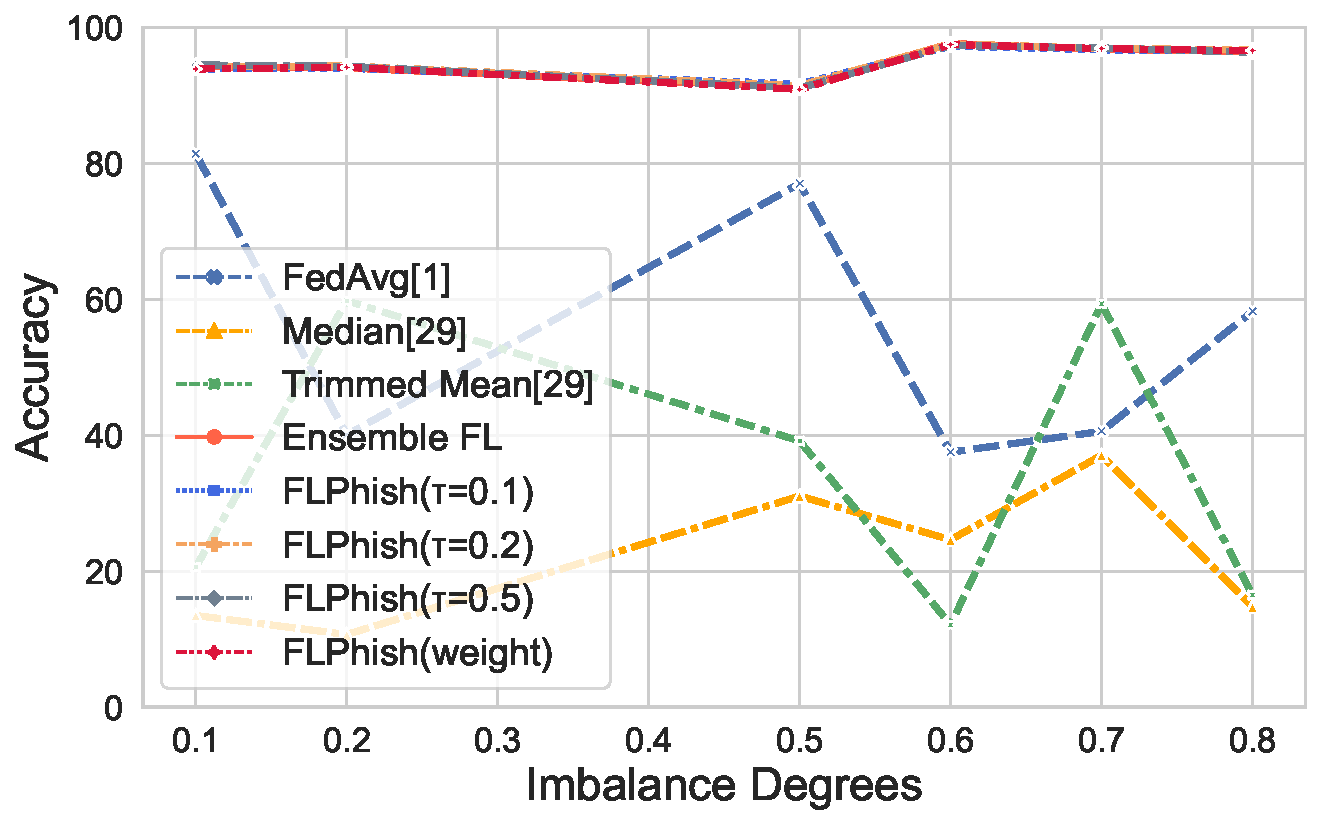
\includegraphics[width=0.24\textwidth]{figures/table_random_imbalances_MNIST.pdf}}
      \subfigure[$q\,0.2$ \& Different $p$]{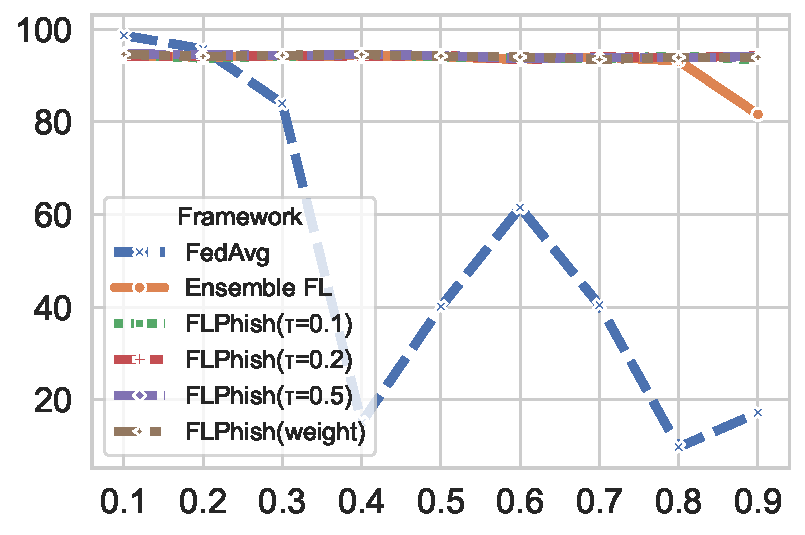
\includegraphics[width=0.24\textwidth]{figures/table_random_byzantines_MNIST.pdf}}
    \\
    \caption{Accuracy values on MNIST under Random Attack.}
    \label{fig_table_mnist_random}
    \vspace{0.2in}
  \end{figure}
  \begin{figure}[!htp]
    \centering
      \subfigure[$p\,0.5$ \& Different $q$]{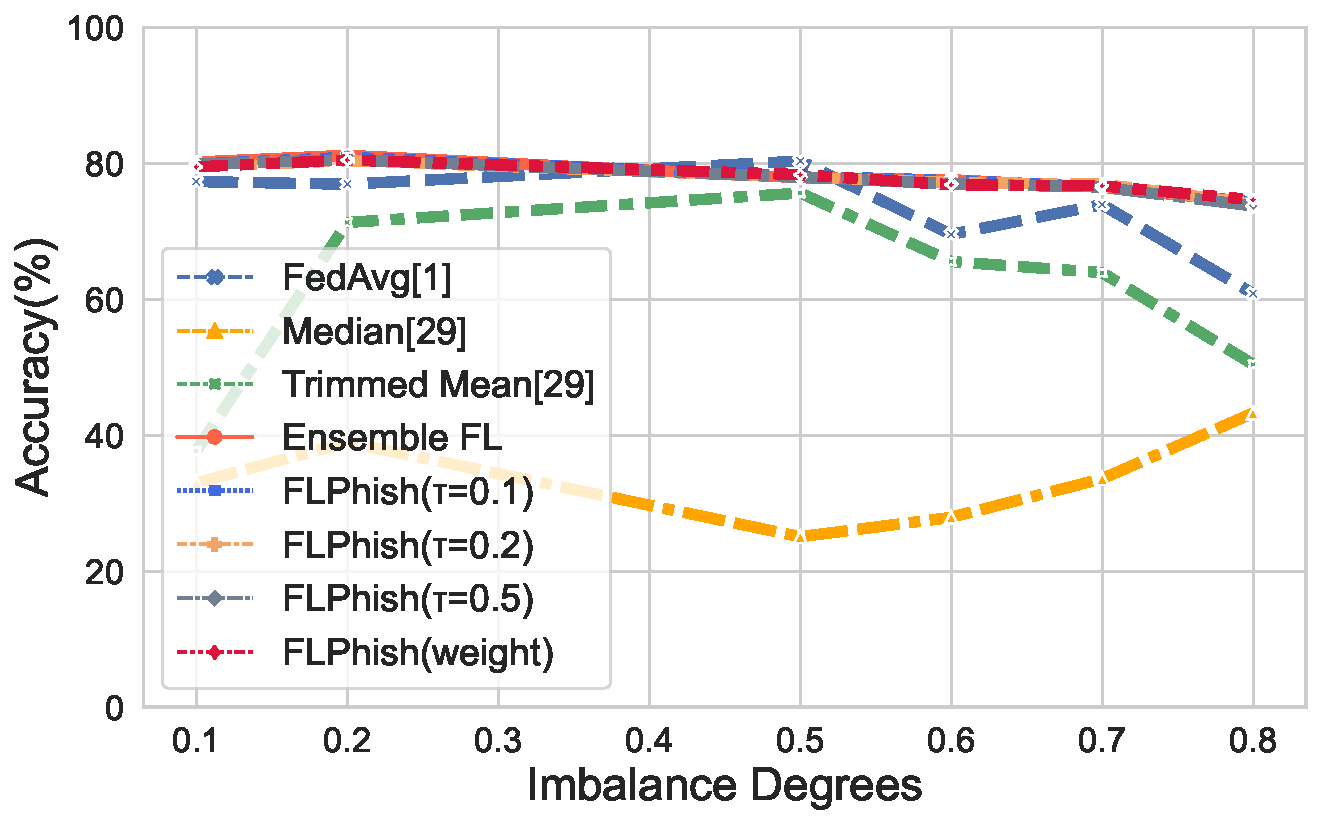
\includegraphics[width=0.24\textwidth]{figures/table_random_imbalances_Fashion-MNIST.pdf}}
      \subfigure[$q\,0.2$ \& Different $p$]{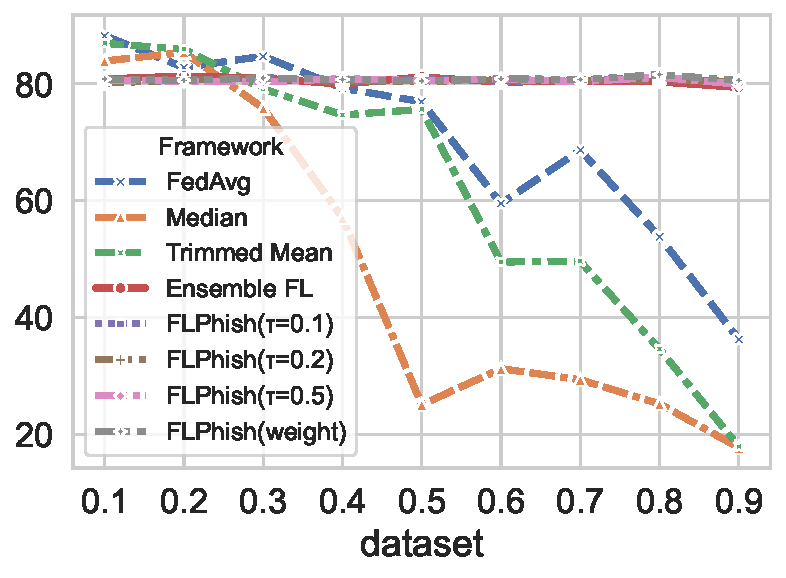
\includegraphics[width=0.24\textwidth]{figures/table_random_byzantines_Fashion-MNIST.pdf}}
    \\
    \caption{Accuracy values on Fashion-MNIST under Random Attack.}
    \label{fig_table_fashion_random}
    \vspace{0.2in}
  \end{figure}
  \begin{figure}[!htp]
    \centering
      \subfigure[$p\,0.5$ \& Different $q$]{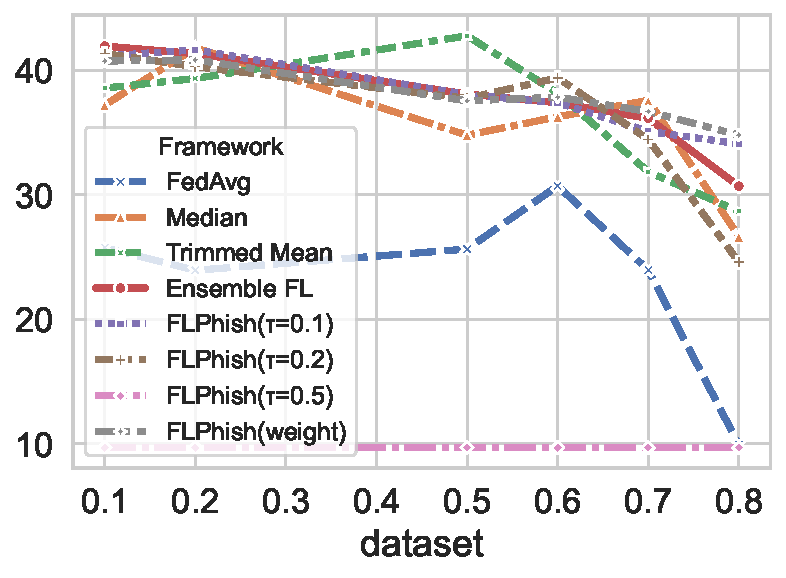
\includegraphics[width=0.24\textwidth]{figures/table_random_imbalances_Cifar-10.pdf}}
      \subfigure[$q\,0.2$ \& Different $p$]{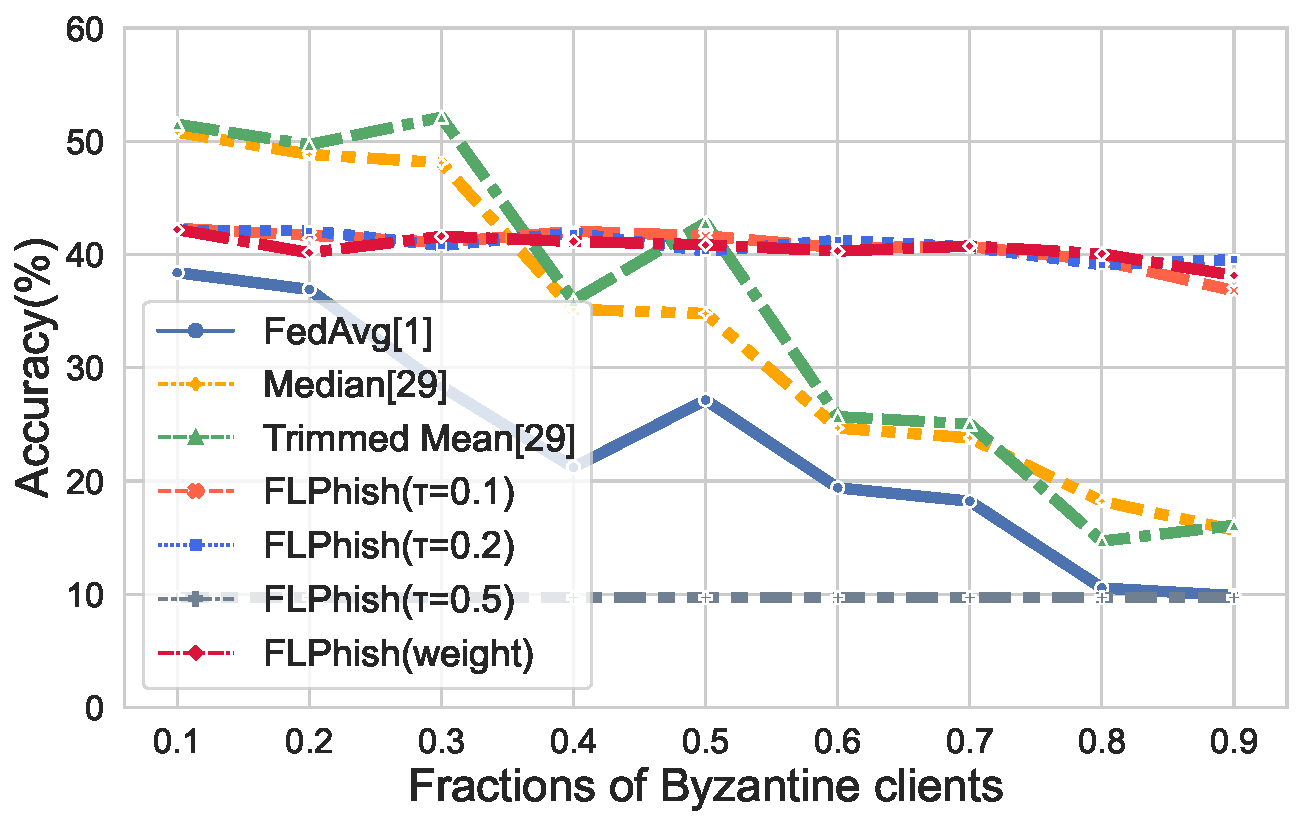
\includegraphics[width=0.24\textwidth]{figures/table_random_byzantines_Cifar-10.pdf}}
    \\
    \caption{Accuracy values on CIFAR-10 under Random Attack.}
    \label{fig_table_cifar_random}
    \vspace{0.2in}
  \end{figure}





  \subsection{{Performance Comparison under Untargeted Attacks}} We further evaluate FLPhish towards untargeted Byzantine attacks in Ensemble FL.
  

  
    \subsubsection{\ul{Performance Comparison with Different Distributions}} We evaluate our FLPhish-threshold and FLPhish-weight under the condition where the Byzantine client portion is a fixed value of 0.5 and distribution imbalance value $q$ is different across the Experiments. The experiment results are shown in Fig. \ref{fig_table_mnist_untargeted}-\ref{fig_table_cifar_untargeted}. We can observe that both the FLPhish-threshold and FLPhish-weight outperform baseline until the imbalance degree $q$ reaches 0.8. The imbalance degree $q$ of 0.8 means that the distribution of data becomes extremely non-IID. The performance of the FLPhish-threshold with a threshold of 0.5 rapidly falls in this case. When facing the distribution of imbalance degree $q=0.8$, each client performs badly, bringing a decline to its reputation. The rise of imbalance degree brings an explosive decline to the global model's accuracy. The accuracy of the global model under the FLPhish-threshold of threshold 0.5 stays 0.1 in the whole learning process. It means that the FLPhish-threshold of threshold 0.5 identifies all the clients as Byzantine clients, making the aggregation process invalid. We can see that the FLPhish-threshold of threshold 0.2 outperforms others. When the distribution becomes non-IID, the threshold of FLPhish-threshold should be set to a lower value to avoid a high false-negative rate. In the experiment of MNIST, it should be set to 0.2. Meanwhile, the performance of FLPhish-weight remains stable under different imbalance degrees.
    
      \begin{figure}[tp]
    \centering
      \subfigure[$p\,0.5$ \& Different $q$]{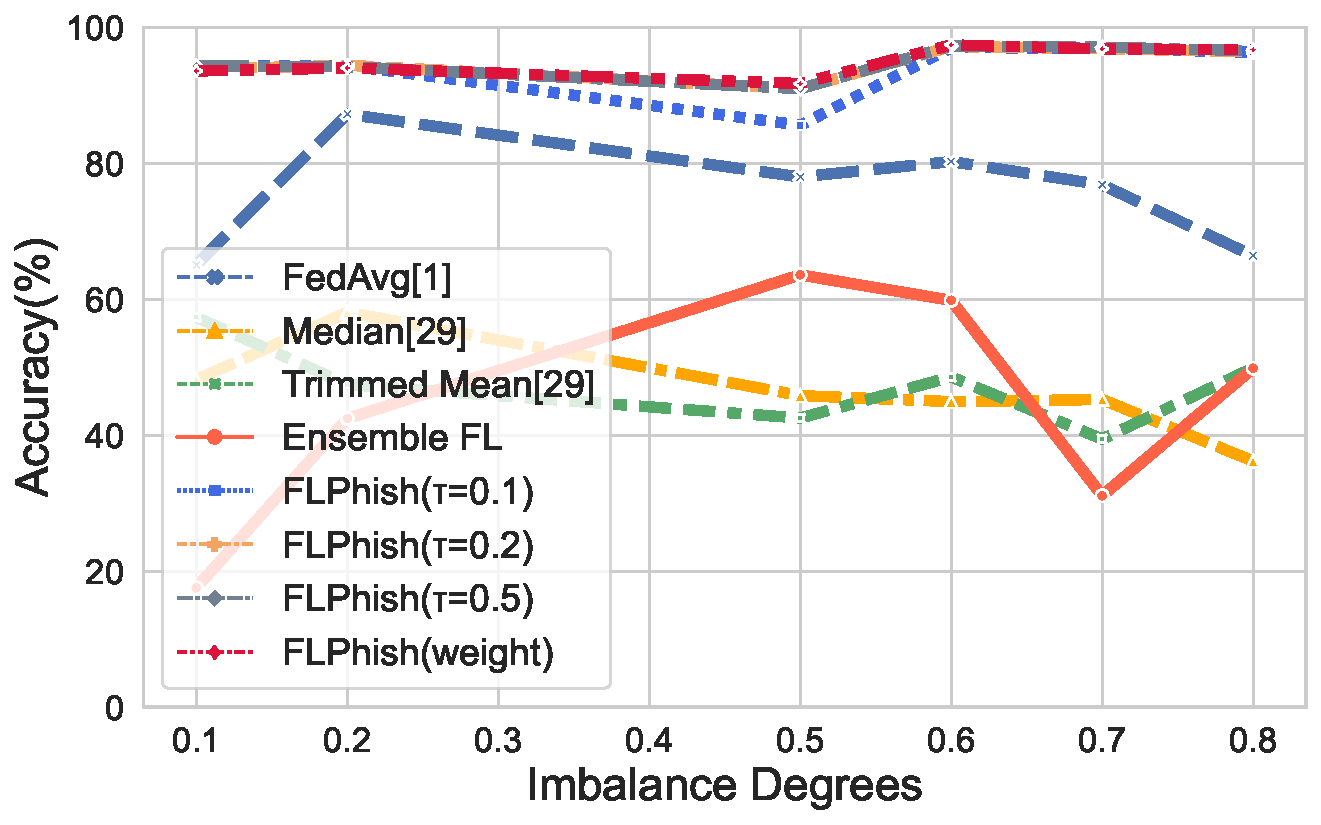
\includegraphics[width=0.24\textwidth]{figures/table_untargeted_imbalances_MNIST.pdf}}
      \subfigure[$q\,0.2$ \& Different $p$]{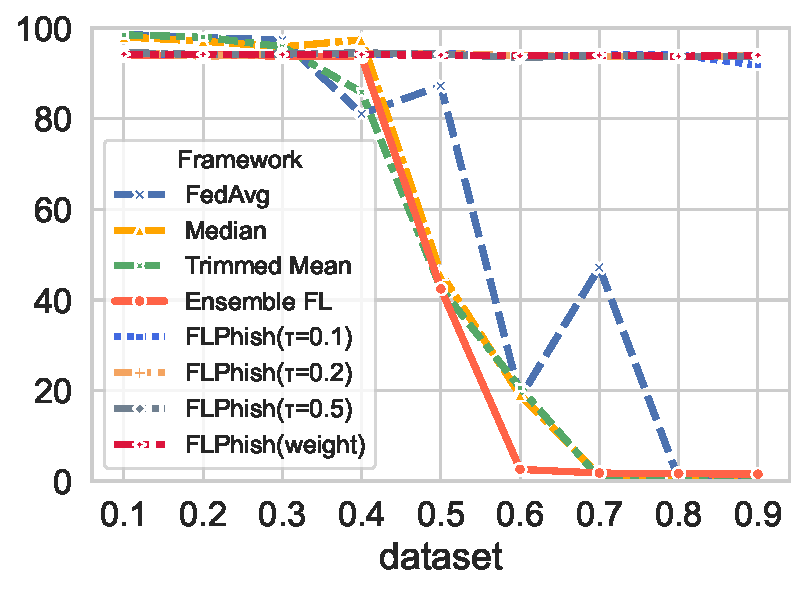
\includegraphics[width=0.24\textwidth]{figures/table_untargeted_byzantines_MNIST.pdf}}
    \\
    \caption{Accuracy values on MNIST under Untargeted Attack.}
    \label{fig_table_mnist_untargeted}
    \vspace{0.2in}
  \end{figure}
  \begin{figure}[tp]
    \centering
      \subfigure[$p\,0.5$ \& Different $q$]{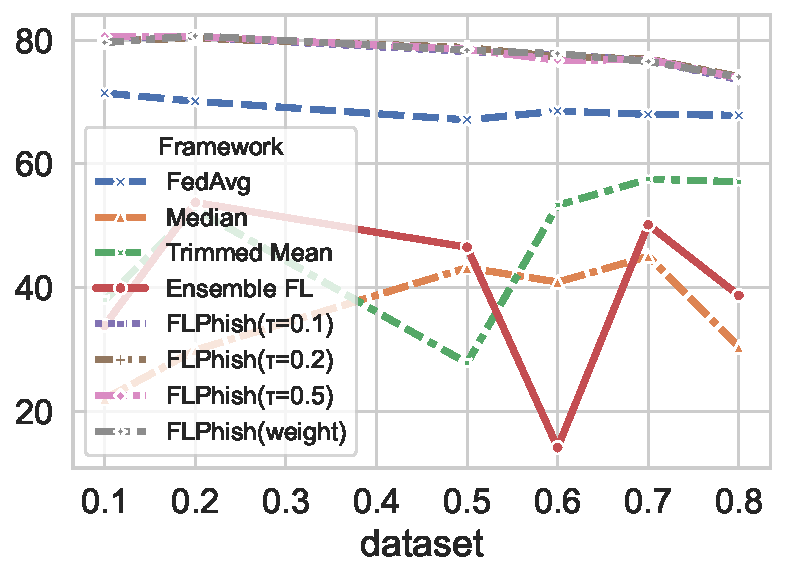
\includegraphics[width=0.24\textwidth]{figures/table_untargeted_imbalances_Fashion-MNIST.pdf}}
      \subfigure[$q\,0.2$ \& Different $p$]{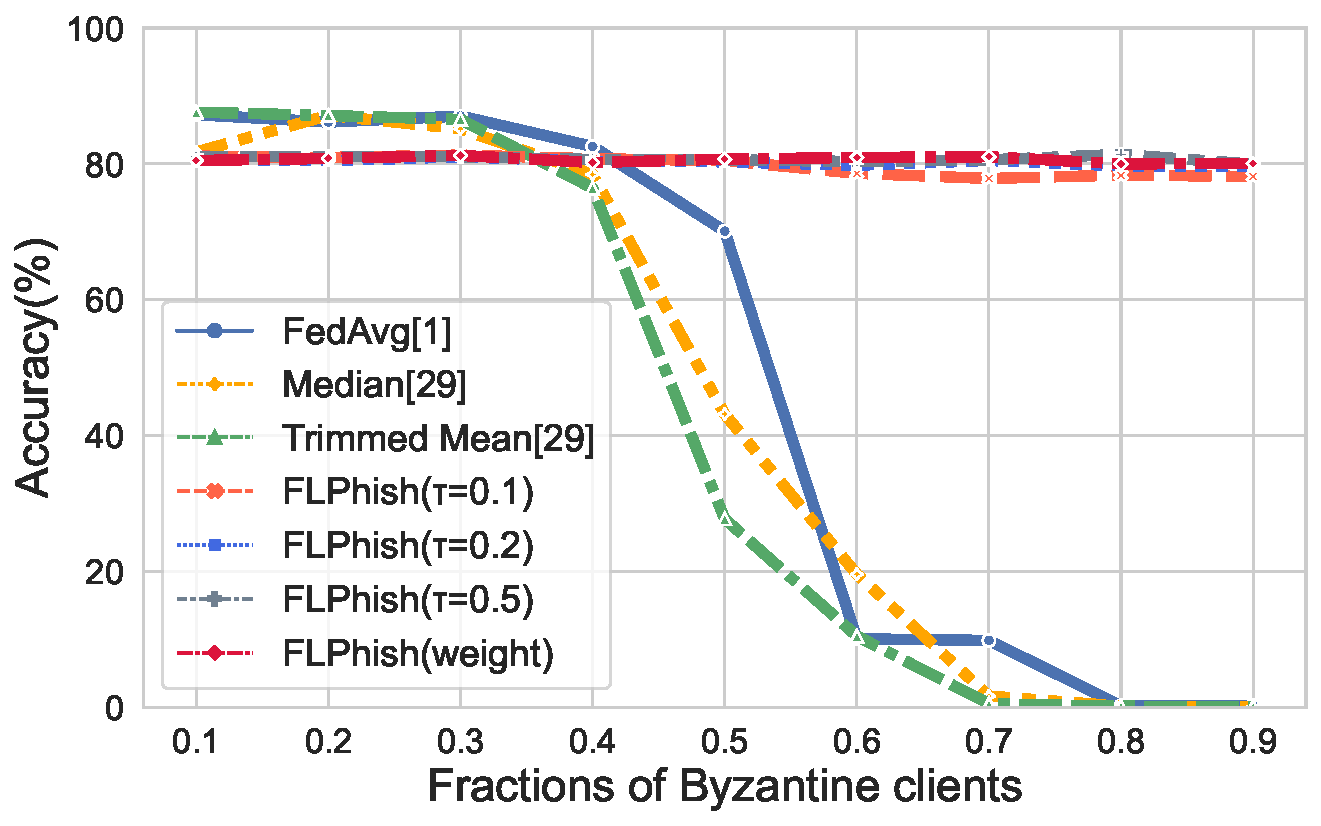
\includegraphics[width=0.24\textwidth]{figures/table_untargeted_byzantines_Fashion-MNIST.pdf}}
    \\
    \caption{Accuracy values on Fashion-MNIST under Untargeted Attack.}
    \label{fig_table_fashion_untargeted}
    \vspace{0.2in}
  \end{figure}
  \begin{figure}[tp]
    \centering
      \subfigure[$p\,0.5$ \& Different $q$]{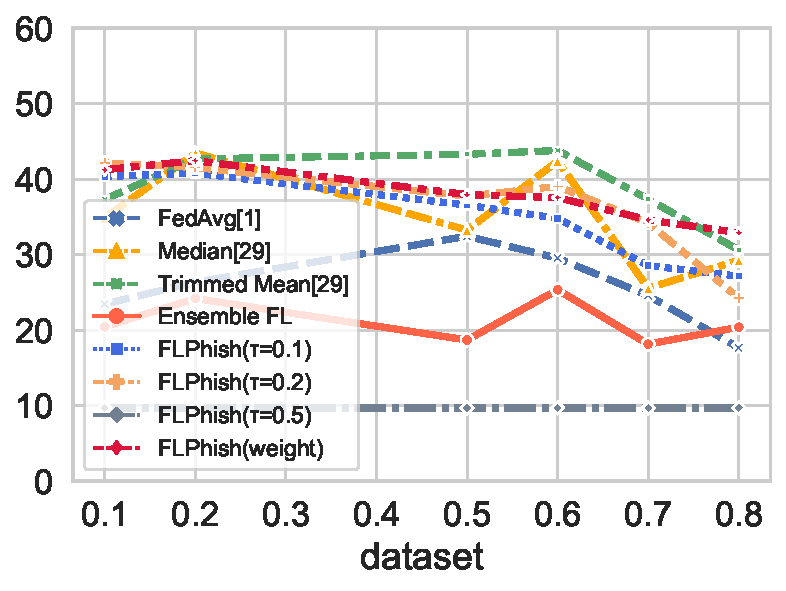
\includegraphics[width=0.24\textwidth]{figures/table_untargeted_imbalances_Cifar-10.pdf}}
      \subfigure[$q\,0.2$ \& Different $p$]{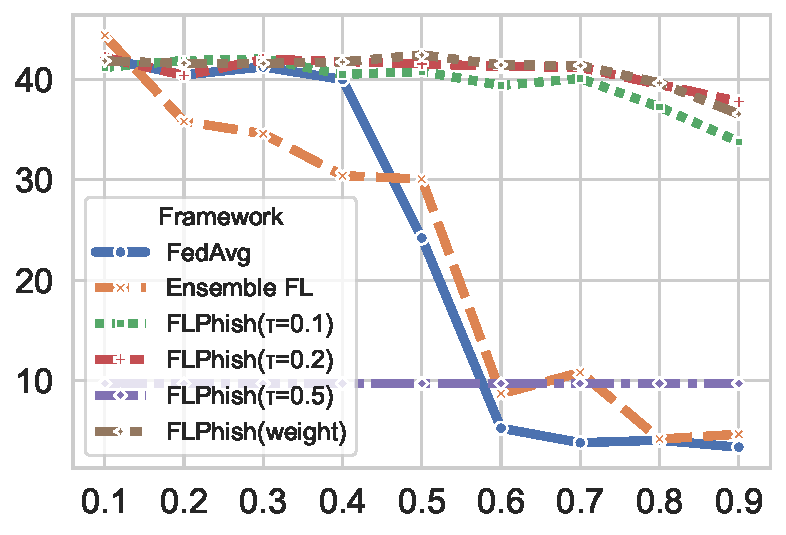
\includegraphics[width=0.24\textwidth]{figures/table_untargeted_byzantines_Cifar-10.pdf}}
    \\
    \caption{Accuracy values on CIFAR-10 under Untargeted Attack.}
    \label{fig_table_cifar_untargeted}
    \vspace{0.2in}
  \end{figure}  
    
    \subsubsection{\ul{Performance Comparison with Different Fractions of Byzantine Clients}} Different fractions of Byzantine clients are taken into account as well. Figure. \ref{fig_table_mnist_untargeted}-\ref{fig_table_cifar_untargeted} shows that the accuracy for FedAvg, Median, Trimmed Mean, and Ensemble FL without any defense mechanisms begins to fall rapidly when the Byzantine portion reaches nearly 50\%. Furthermore, FedAvg, Median, and Trimmed Mean perform extremely invalidly (the accuracy falls below 1\%) when encountered with high fractions of Byzantine attackers. In comparison, FLPhish's (including FLPhish-threshold and FLPhish-weight) performance under various thresholds maintains a high level of performance as the portion grows. Both FLPhish-threshold and FLPhish-weight effectively detect Byzantine clients and accurately discards them from the aggregation process. The global model can be successfully trained without the involvement of Byzantine clients in aggregation procedures. Furthermore, the data show that FLPhish-threshold with a 0.1 threshold performs worse than the other two. This is since the 0.1 threshold is far too low to adequately detect Byzantine clients. Though the Byzantine attackers will try to make the right predictions of the public dataset and then send the opposite wrong predictions to the FL server. But they will also make wrong predictions first and coincidentally transfer the opposite right predictions to the FL server. Thus the reputation values of some Byzantine clients, in particular, can exceed 0.1. It indicates that if the threshold is not well set, Byzantine clients can avoid being detected by FLPhish-threshold. As the fractions of Byzantine clients go over the threshold of 50\%, the harm brought by untargeted Byzantine attacks will increase rapidly for they outnumber the fractions of the benign clients. In the meantime, FLPhish-weight shows stable performance whenever the fractions of Byzantine clients are.

    \subsection{{Experiment Result Analysis}} Our experiment results demonstrate that both FLPhish-threshold and FLPhish-weight outperform FedAvg, Median \cite{ref_13_defense} and Trimmed Mean \cite{ref_13_defense} on defending against Byzantine attacks in FL. The results also show that the FLPhish-threshold's setting threshold value has a significant impact on the performance of the FLPhish-threshold. Only when the managers of FL servers have complete knowledge of FL clients (the imbalance degree of each client), can they accurately set the value of the threshold suitably. However, it is not feasible due to the privacy concern of FL. FLPhish-weight, on the other hand, remains constant regardless of the circumstances. FLPhish-weight can let clients with higher performance have a stronger influence on the aggregation process by using the reputation value as the weight. To summarize, FLPhish-weight is a better and more stable aggregation technique than FLPhish-threshold and is a more practical Byzantine defense framework.






\section{Conclusion}

In this paper, we have designed an FL architecture, Ensemble Federated Learning in this study, which allows us to use the unlabeled dataset to transfer knowledge between the FL server and FL clients. We have crafted the FLPhish technique to make Ensemble FL resistant to Byzantine attacks by using a labeled dataset as `bait' to detect malicious Byzantine clients. Furthermore, we have proposed a reputation technique based on Bayesian inference for determining a client's level of trust. We have also presented two aggregation techniques, FLPhish-threshold and FLPhish-weight, to improve FLPhish's performance. At last, we have tested our suggested FLPhish in a variety of scenarios. The results of the experiment reveal that FLPhish performs admirably against Byzantine attacks. Even when confronted with very non-IID distributions and high fractions of Byzantine clients, FLPhish outperforms FedAvg and Ensemble FL significantly.
\par Our future work will evaluate FLPhish against more advanced Byzantine attacks and improve our framework based on the evaluation results.

\bibliography{IEEEabbrv}
\bibliographystyle{IEEEtran}






% that's all folks
\end{document}